\chapter{Experiments and Results}
\label{sec:experiments}
In this section, various experiments are performed in order to gauge the effectiveness of Grid HTM. There are three experiments in total, and each experiment covers a different use case. For reproducibility purposes, each experiment has corresponding tables of the parameters used.
\section{Bouncing Ball Experiment}
To give credibility to the approach mentioned in \autoref{sec:grid_htm}, a simple experiment to test the capabilities of \gls*{htm} and confirm that they apply on a video is introduced.
\subsection{Data}
\begin{figure}[H]
    \centering
    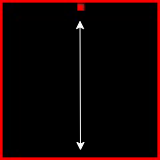
\includegraphics[width=.3\textwidth]{resources/experiments/bouncing_ball/bb_updown1.png}\hfill
    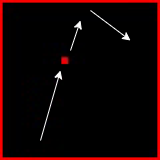
\includegraphics[width=.3\textwidth]{resources/experiments/bouncing_ball/bb_updownside.png}\hfill
    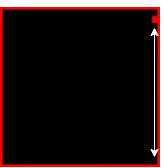
\includegraphics[width=.3\textwidth]{resources/experiments/bouncing_ball/bb_updown2.png}
    \caption[Bouncing Ball Experiment]{The bouncing ball experiment, and its three stages.}
    \label{fig:bb}
\end{figure}
The video consists of a ball bouncing up and down until an anomaly occurs in the form of a sudden introduction of a horizontal velocity. After a while this horizontal velocity is set back to 0 and the ball is once again bouncing up and down in-place. This is visualized in \autoref{fig:bb}.
\par
\subsection{HTM}
The model used is a standard \gls*{htm} model, which covers the entire input. This is equivalent to a single cell in a Grid HTM.
\begin{figure}[H]
    \centering
    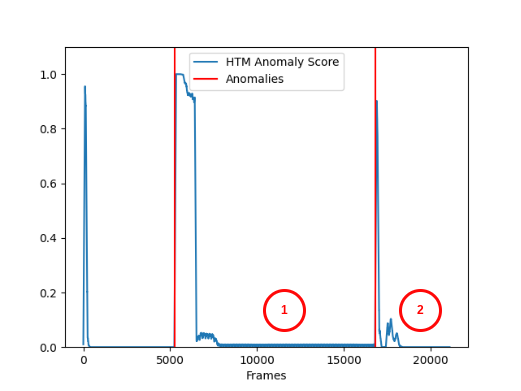
\includegraphics[width=0.9\textwidth]{resources/experiments/bouncing_ball/bb_anoms_bad.png}
    \caption[Bouncing Ball Experiment Anomaly Score]{The anomaly score in the bouncing ball experiment.}
    \label{fig:bb_normal}
\end{figure}
From \autoref{fig:bb_normal} it can be observed that \gls*{htm} correctly detects anomalies and quickly adapts to them. On the other hand, the result is not perfect due to the minor oscillations close to $(1)$ and the anomaly spikes towards the end close to $(2)$. While the imperfections are not major and can be safely ignored, it is still important to understand their causes and what can be done to improve upon them. \par
\subsubsection{Boosting}
The reason for the oscillations is due to the spatial pooler being dominated by a lucky few columns. The solution is to enable boosting, as explained in \autoref{sec:spatial_pooler}. This also helped with the spikes towards the end, as can be seen in \autoref{fig:bb_boosting}.\par
\begin{figure}[H]
    \centering
    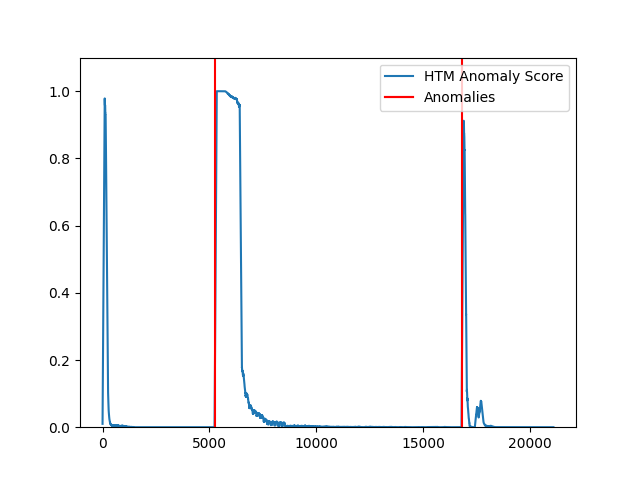
\includegraphics[width=0.9\textwidth]{resources/experiments/bouncing_ball/bb_anoms_boosting.png}
    \caption[Bouncing Ball Experiment Anomaly Score No Boosting]{Bouncing ball with boosting enabled.}
    \label{fig:bb_boosting}
\end{figure}
\subsubsection{Zero Permanence Decrement}
The reason for the anomaly spikes towards the end is because the spatial pooler has found an optimal representation when the ball is bouncing freely, but when the ball stops and starts bouncing in-place the spatial pooler ends up unlearning the old optimal representation while it learns the new optimal representation. This causes a sudden minor change in the \gls*{sp} output, which the \gls*{tm} reports as anomalous.
\par
The solution is to set the value by which permanence is decreased by to zero, effectively disabling the ability of the spatial pooler to "forget", as can be seen in \autoref{fig:bb_forget}. That being said, the ability to decrement permanence is important in \gls*{htm} systems, therefore disabling it is not always feasible.
\begin{figure}[H]
    \centering
    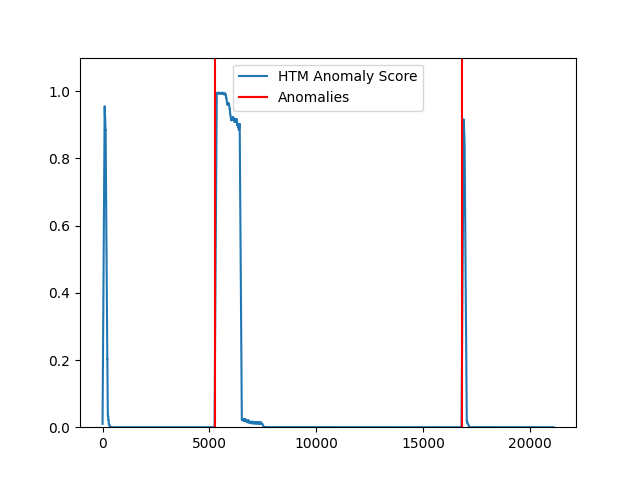
\includegraphics[width=0.9\textwidth]{resources/experiments/bouncing_ball/bb_anoms_unforgetting.png}
    \caption[Bouncing Ball Experiment Anomaly Score Zero Decrement]{Bouncing ball without the ability of the \gls*{sp} to "forget".}
    \label{fig:bb_forget}
\end{figure}
\subsubsection{Boosting and Zero Permanence Decrement}
Finally, for the sake of interest, the bouncing ball example was performed with both boosting enabled and with zero permanence decrement. Results can be seen in \autoref{fig:bb_boosting_forget}.
\begin{figure}[H]
    \centering
    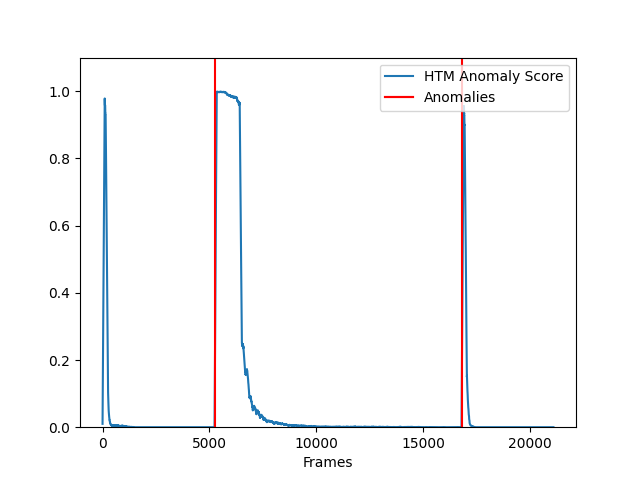
\includegraphics[width=0.9\textwidth]{resources/experiments/bouncing_ball/bb_anoms_unforgetting_boosting.png}
    \caption[Bouncing Ball Experiment Anomaly Score No Boosting Zero Decrement]{Bouncing ball without the ability of the \gls*{sp} to "forget" and with boosting enabled.}
    \label{fig:bb_boosting_forget}
\end{figure}
\subsubsection{Parameters}
Final list of parameters for reproducibility. For the plots, a moving average of $n=100$ was used to smooth the output.
\begin{table}[H]
    \centering
    \begin{tabularx}{\linewidth}{@{}llX@{}}
        \toprule
        \textbf{Parameter} & \textbf{Value} & \textbf{Notes}                                             \\
        \midrule
        inputDimensions    & 120, 120       & The shape of the entire frame                              \\
        columnDimensions   & 60, 60         &                                                            \\
        potentialPct       & 0.1            &                                                            \\
        potentialRadius    & 120            &                                                            \\
        localAreaDensity   & 0.02           &                                                            \\
        globalInhibition   & True           & Set to False to enable topology                            \\
        wrapAround         & True           &
        Allows the columns near the edges to "wrap around" and form connections on the other side        \\
        synPermActiveInc   & 0.1            &                                                            \\
        synPermInactiveDec & 0              & Set to \textgreater{}0 to enable the \gls*{sp} to "forget" \\
        stimulusThreshold  & 2              &                                                            \\
        seed               & 2              &                                                            \\
        boostStrength      & 0.1            & Set to 0 to disable boosting                               \\
        dutyCyclePeriod    & 250            &                                                            \\
        \bottomrule
    \end{tabularx}

    \caption{SP Parameters}
    \label{tab:bb_sp_params}
\end{table}
\begin{table}[H]
    \centering
    \begin{tabularx}{\linewidth}{@{}llX@{}}
        \toprule
        \textbf{Parameter}        & \textbf{Value} & \textbf{Notes}        \\
        \midrule
        columnDimensions          & 60, 60         & Same as the \gls*{sp} \\
        predictedSegmentDecrement & 0.003          &                       \\
        permanenceIncrement       & 0.1            &                       \\
        permanenceDecrement       & 0.001          &                       \\
        minThreshold              & 3              &                       \\
        activationThreshold       & 5              &                       \\
        cellsPerColumn            & 16             &                       \\
        seed                      & 2              &                       \\
        \bottomrule
    \end{tabularx}

    \caption{TM Parameters}
    \label{tab:bb_TM_params}
\end{table}
\subsection{Grid HTM}
This is a very simple problem which does not require invariances, making it unsuitable for Grid HTM. Grid \gls*{htm} would be suitable if there were two or more independent bouncing balls, due to its improved invariance. Still, it is interesting to see how Grid \gls*{htm} performs compared to normal HTM.
\subsubsection{Results}
\begin{figure}[H]
    \centering
    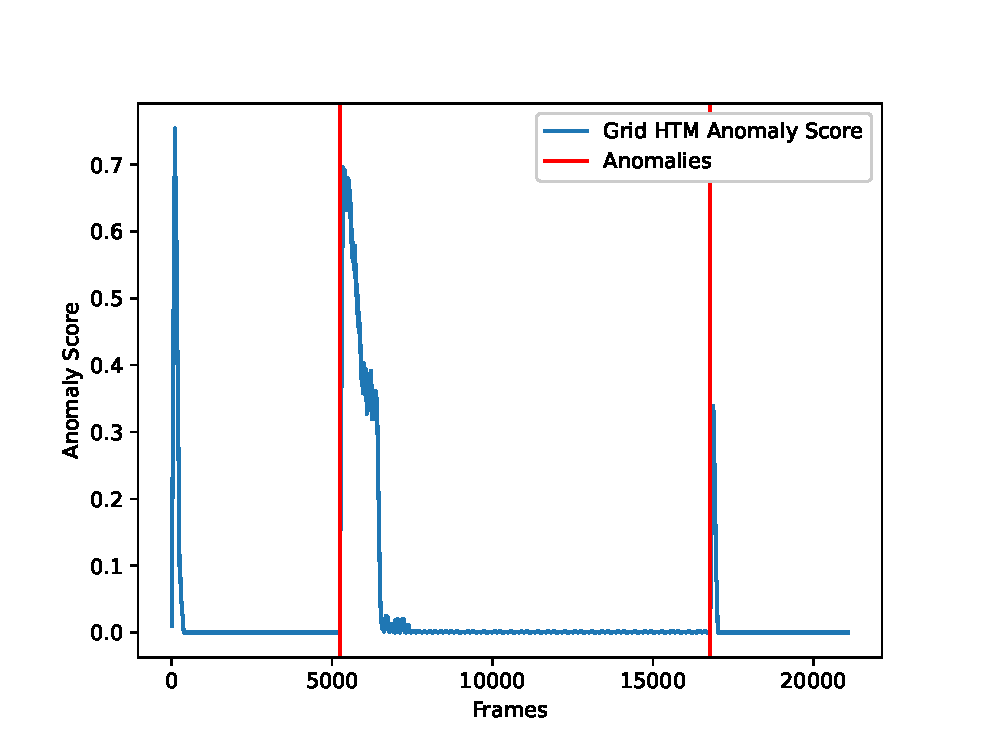
\includegraphics[width=0.9\textwidth]{resources/experiments/bouncing_ball/bb_grid}
    \caption[Bouncing Ball Experiment Anomaly Score Grid HTM]{Results when using Grid HTM}
    \label{fig:bb_gridhtm}
\end{figure}
It can be observed in \autoref{fig:bb_gridhtm} that Grid \gls*{htm} performs worse than the normal HTM, but the result is still acceptable. This is to be expected since this problem is not suited for Grid HTM, and that the parameters given in \autoref{tab:bb_gridhtm_params}, \autoref{tab:bb_sp_gridhtm_param}, and \autoref{tab:bb_tm_gridhtm_param} are probably not optimal.
\subsubsection{Parameters}
The \gls*{sp} and \gls*{tm} parameters were selected so that they were as close as possible to the normal \gls*{htm} parameters. The non-zero mean was chosen as the aggregation function, because there is no noise due to the controlled environment. Again, a moving average of $n=100$ was used to smooth the anomaly score output in the plots.
\begin{table}[H]
    \centering
    \begin{tabularx}{\linewidth}{@{}XlX@{}}
        \toprule
        \textbf{Parameter} & \textbf{Value} & \textbf{Notes}                                                             \\
        \midrule
        sp\_grid\_size     & 30, 30         & Size of each grid                                                          \\
        tm\_grid\_size     & 15, 15         & Size of each \gls*{sp} grid output.                                        \\
        min\_sparsity      & 1              &                                                                            \\
        sparsity           & A              & Area of the bouncing ball with radius=3                                    \\
        temporal\_size     & 1              & Size of the multistep temporal pattern, 1 means it is effectively disabled \\
        \bottomrule
    \end{tabularx}
    \caption{Grid HTM specific parameters}
    \label{tab:bb_gridhtm_params}
\end{table}
\begin{table}[H]
    \centering
    \begin{tabularx}{\linewidth}{@{}XlX@{}}
        \toprule
        \textbf{Parameter} & \textbf{Value} & \textbf{Notes}                                                  \\
        \midrule
        inputDimensions    & sp\_grid\_size &                                                                 \\
        columnDimensions   & tm\_grid\_size &                                                                 \\
        potentialPct       & 0.5            & Increased in order to compensate for the smaller potential pool \\
        potentialRadius    & 5              &                                                                 \\
        localAreaDensity   & 0.1            &                                                                 \\
        globalInhibition   & True           & Set to False to enable topology                                 \\
        wrapAround         & False          &                                                                 \\
        synPermActiveInc   & 0.1            &                                                                 \\
        synPermInactiveDec & 0.001                                                                            \\
        stimulusThreshold  & 2              &                                                                 \\
        boostStrength      & 0              & Causes instability in empty cells                               \\
        \bottomrule
    \end{tabularx}
    \caption{SP Parameters}
    \label{tab:bb_sp_gridhtm_param}
\end{table}
\begin{table}[H]
    \centering
    \begin{tabularx}{\linewidth}{@{}XlX@{}}
        \toprule
        \textbf{Parameter}        & \textbf{Value} & \textbf{Notes}        \\
        \midrule
        columnDimensions          & tm\_grid\_size & Same as the \gls*{sp} \\
        predictedSegmentDecrement & 0.003          &                       \\
        permanenceIncrement       & 0.1            &                       \\
        permanenceDecrement       & 0.001          &                       \\
        minThreshold              & 1              &                       \\
        activationThreshold       & 1              &                       \\
        cellsPerColumn            & 16             &                       \\
        \bottomrule
    \end{tabularx}
    \caption{TM Parameters}
    \label{tab:bb_tm_gridhtm_param}
\end{table}
\subsection{Experiment Summary}
This experiment is a controlled experiment involving a computer generated ball bouncing up and down, and then introducing an anomaly in the form of a change in horizontal velocity. Finally, the horizontal velocity is set back to 0. First the experiment is performed with a normal \gls*{htm} model.
\par
The results show that it is capable of detecting the anomalies and quickly adapts to them. The same experiment is then performed with Grid HTM. The results show that Grid \gls*{htm} is also capable of detecting the anomalies and quickly adapts to them, however it performs slightly worse than normal HTM. The reason is that Grid \gls*{htm} is designed for more complex videos, such as if there were multiple bouncing balls at once.
\clearpage
\section{Surveillance Experiment}
As stated earlier, one of the use cases of Grid \gls*{htm} is anomaly detection in surveillance. This example will show how Grid \gls*{htm} could perform.
The video to be used is part of the VIRAT~\cite{VIRAT} video dataset, and was selected due to its long duration and stationary camera, which is shown in \autoref{fig:selected_frame}.
\par
The downside is that the video does not contain any non-technical anomalies, but consists of technical anomalies in the form of several segments with sudden frame skips in between. There is also a synthetic anomaly introduced in the form of a frame repeat lasting a couple of seconds, essentially "freezing" time, in order to test whether Grid \gls*{htm} is able to understand how objects should be moving in time.
\begin{figure}[H]
    \centering
    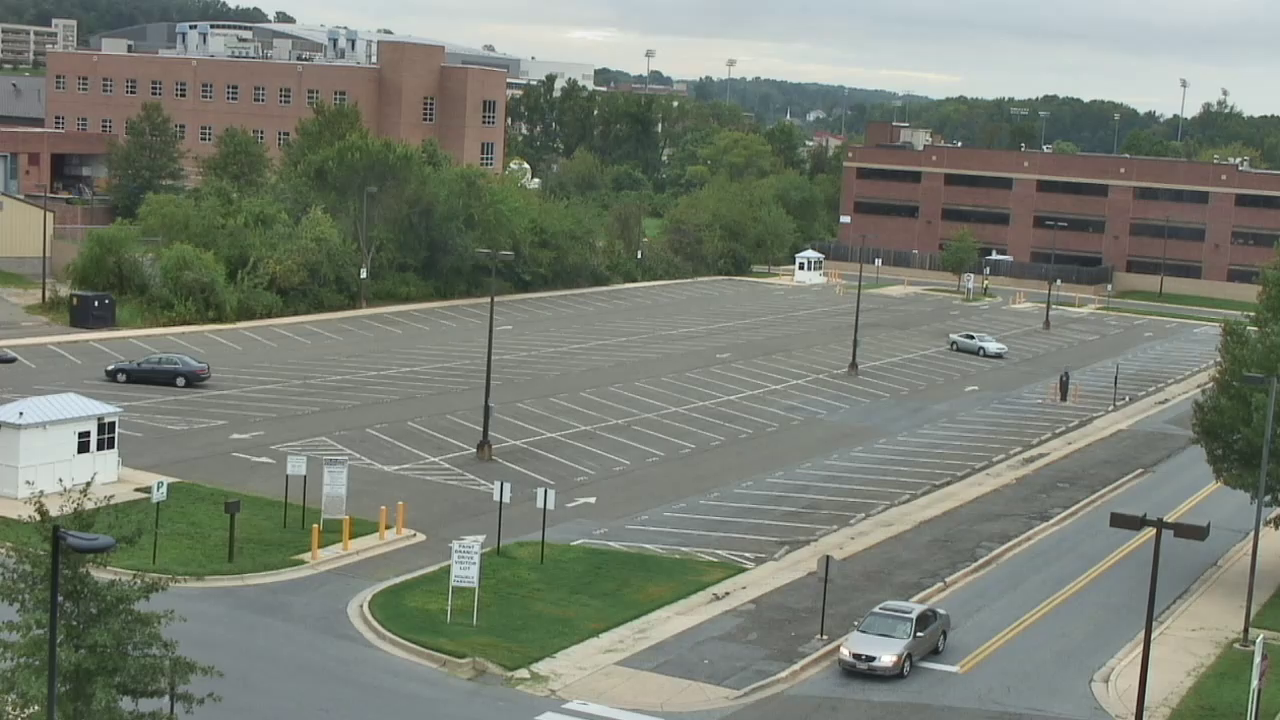
\includegraphics[width=0.8\textwidth]{resources/methodology/original.png}
    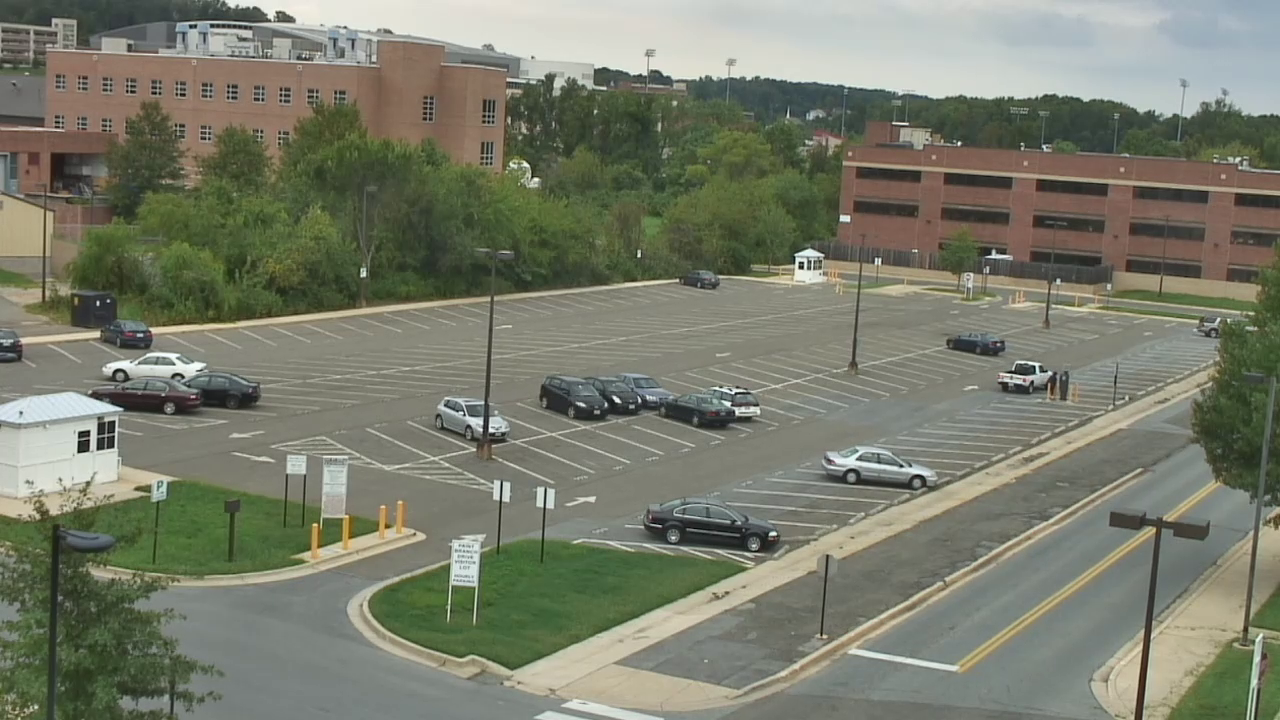
\includegraphics[width=0.8\textwidth]{resources/experiments/surveillance/parking_frame.png}
    \caption[Example Frames]{Example frames from the selected video.}
    \label{fig:selected_frame}
\end{figure}
As previously mentioned, both binary thresholding and deep learning feature map extraction as encoders have their downsides. Therefore, this thesis proposes to use a combination of both, a segmentation model which can extract classes into their respective SDRs. Meaning that there could be an \gls*{sdr} for cars and an \gls*{sdr} for persons (see \autoref{fig:seg_car_person}), that are then concatenated before being fed into the system.
\par
The segmentation model used is PointRend~\cite{pointrend} with a ResNet101~\cite{resnet} backbone, pretrained on ImageNet~\cite{imagenet}, and implemented using PixelLib~\cite{pixellib}.
\begin{figure}[H]
    \centering
    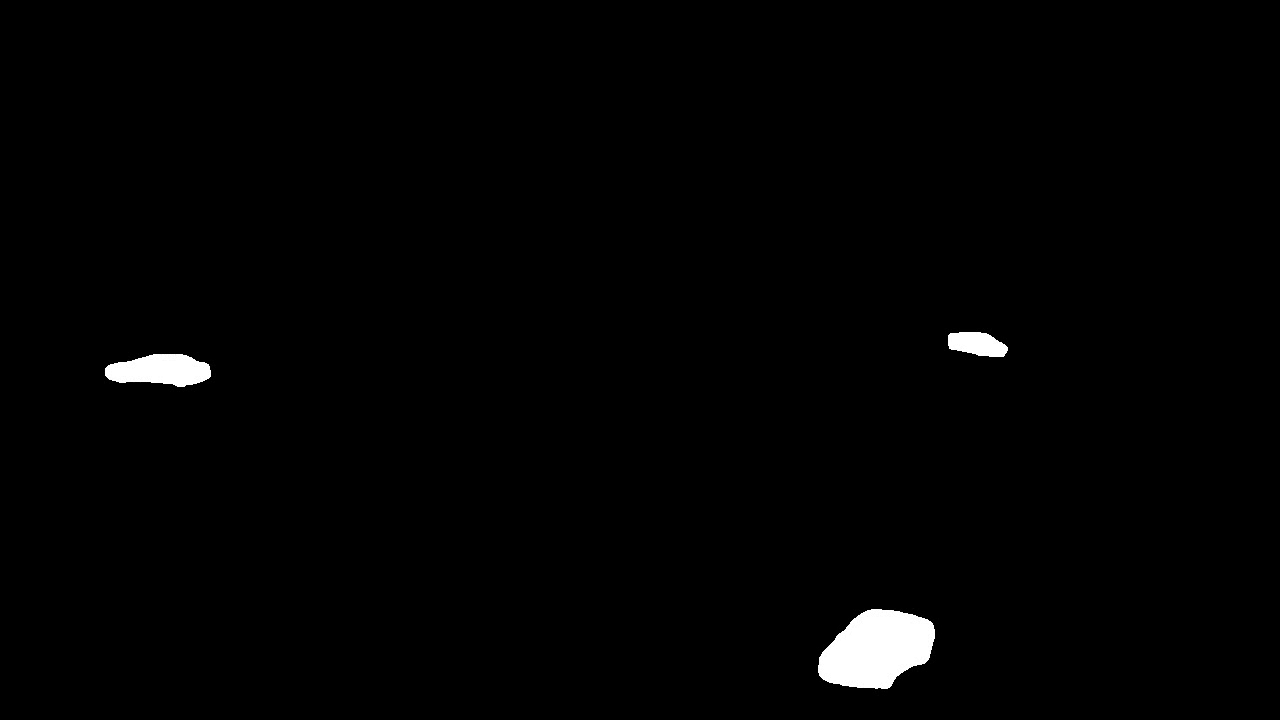
\includegraphics[width=0.45\textwidth]{resources/methodology/car_segmentation.png}
    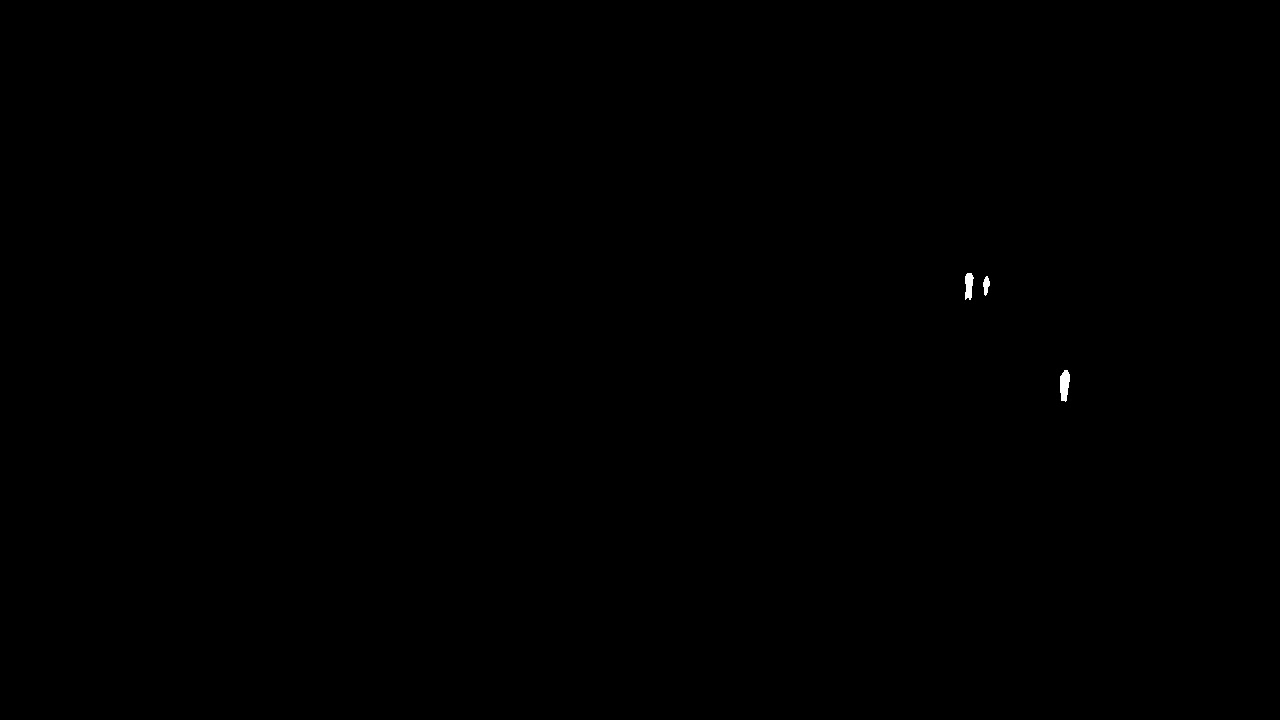
\includegraphics[width=0.45\textwidth]{resources/methodology/person_segmentation.png}
    \caption[Example Segmentation of Cars and Persons]{Example segmentation of cars and persons.}
    \label{fig:seg_car_person}
\end{figure}
For the sake of simplicity, this experiment will focus only on the segmentation of cars.
\par
While on the topic of segmentation, it is important to mention that the segmentation model is not perfect and that there are cases where objects are misclassified as well as cases where cars repeatedly go above and below the confidence threshold.
\subsection{Results}
\begin{figure}[H]
    \centering
    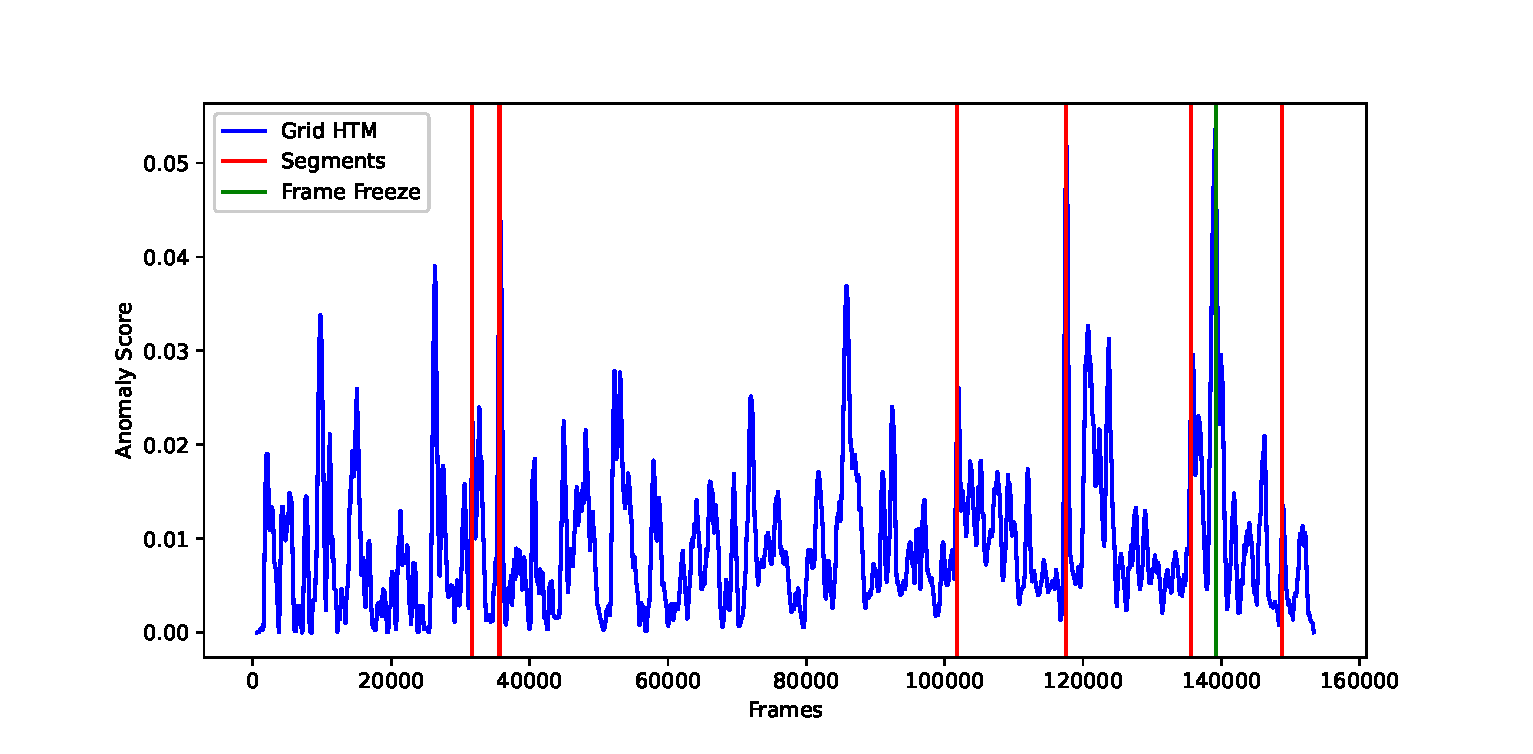
\includegraphics[width=\textwidth]{resources/experiments/surveillance/surveillance_result}
    \caption[Grid HTM Anomaly Score Output]{Anomaly score output from Grid HTM.}
    \label{fig:surveillance_results}
\end{figure}
It can be observed in \autoref{fig:surveillance_results} that Grid \gls*{htm} is detecting when segments begin and end, however it is not possible to use a threshold value to isolate them, and they also have vastly different anomaly scores compared to each other. This is due to the way the aggregation function works, which means that the anomaly output is dependent on the physical size of the anomaly. It should also be noted that a moving average ($n=200$) was applied to smooth out the anomaly score output, otherwise the graph would be too noisy.
\par
With the aggregation functions presented in this thesis in mind, it is safe to conclude that looking at the anomaly score output is meaningless for complex data such as a surveillance video. This however does not mean that Grid \gls*{htm} is completely useless, and this can be observed by looking at the visual output of Grid HTM. The visual output during which the first segment anomaly occurs can be seen in \autoref{fig:surveillance_segment}.
\begin{figure}[H]
    \centering
    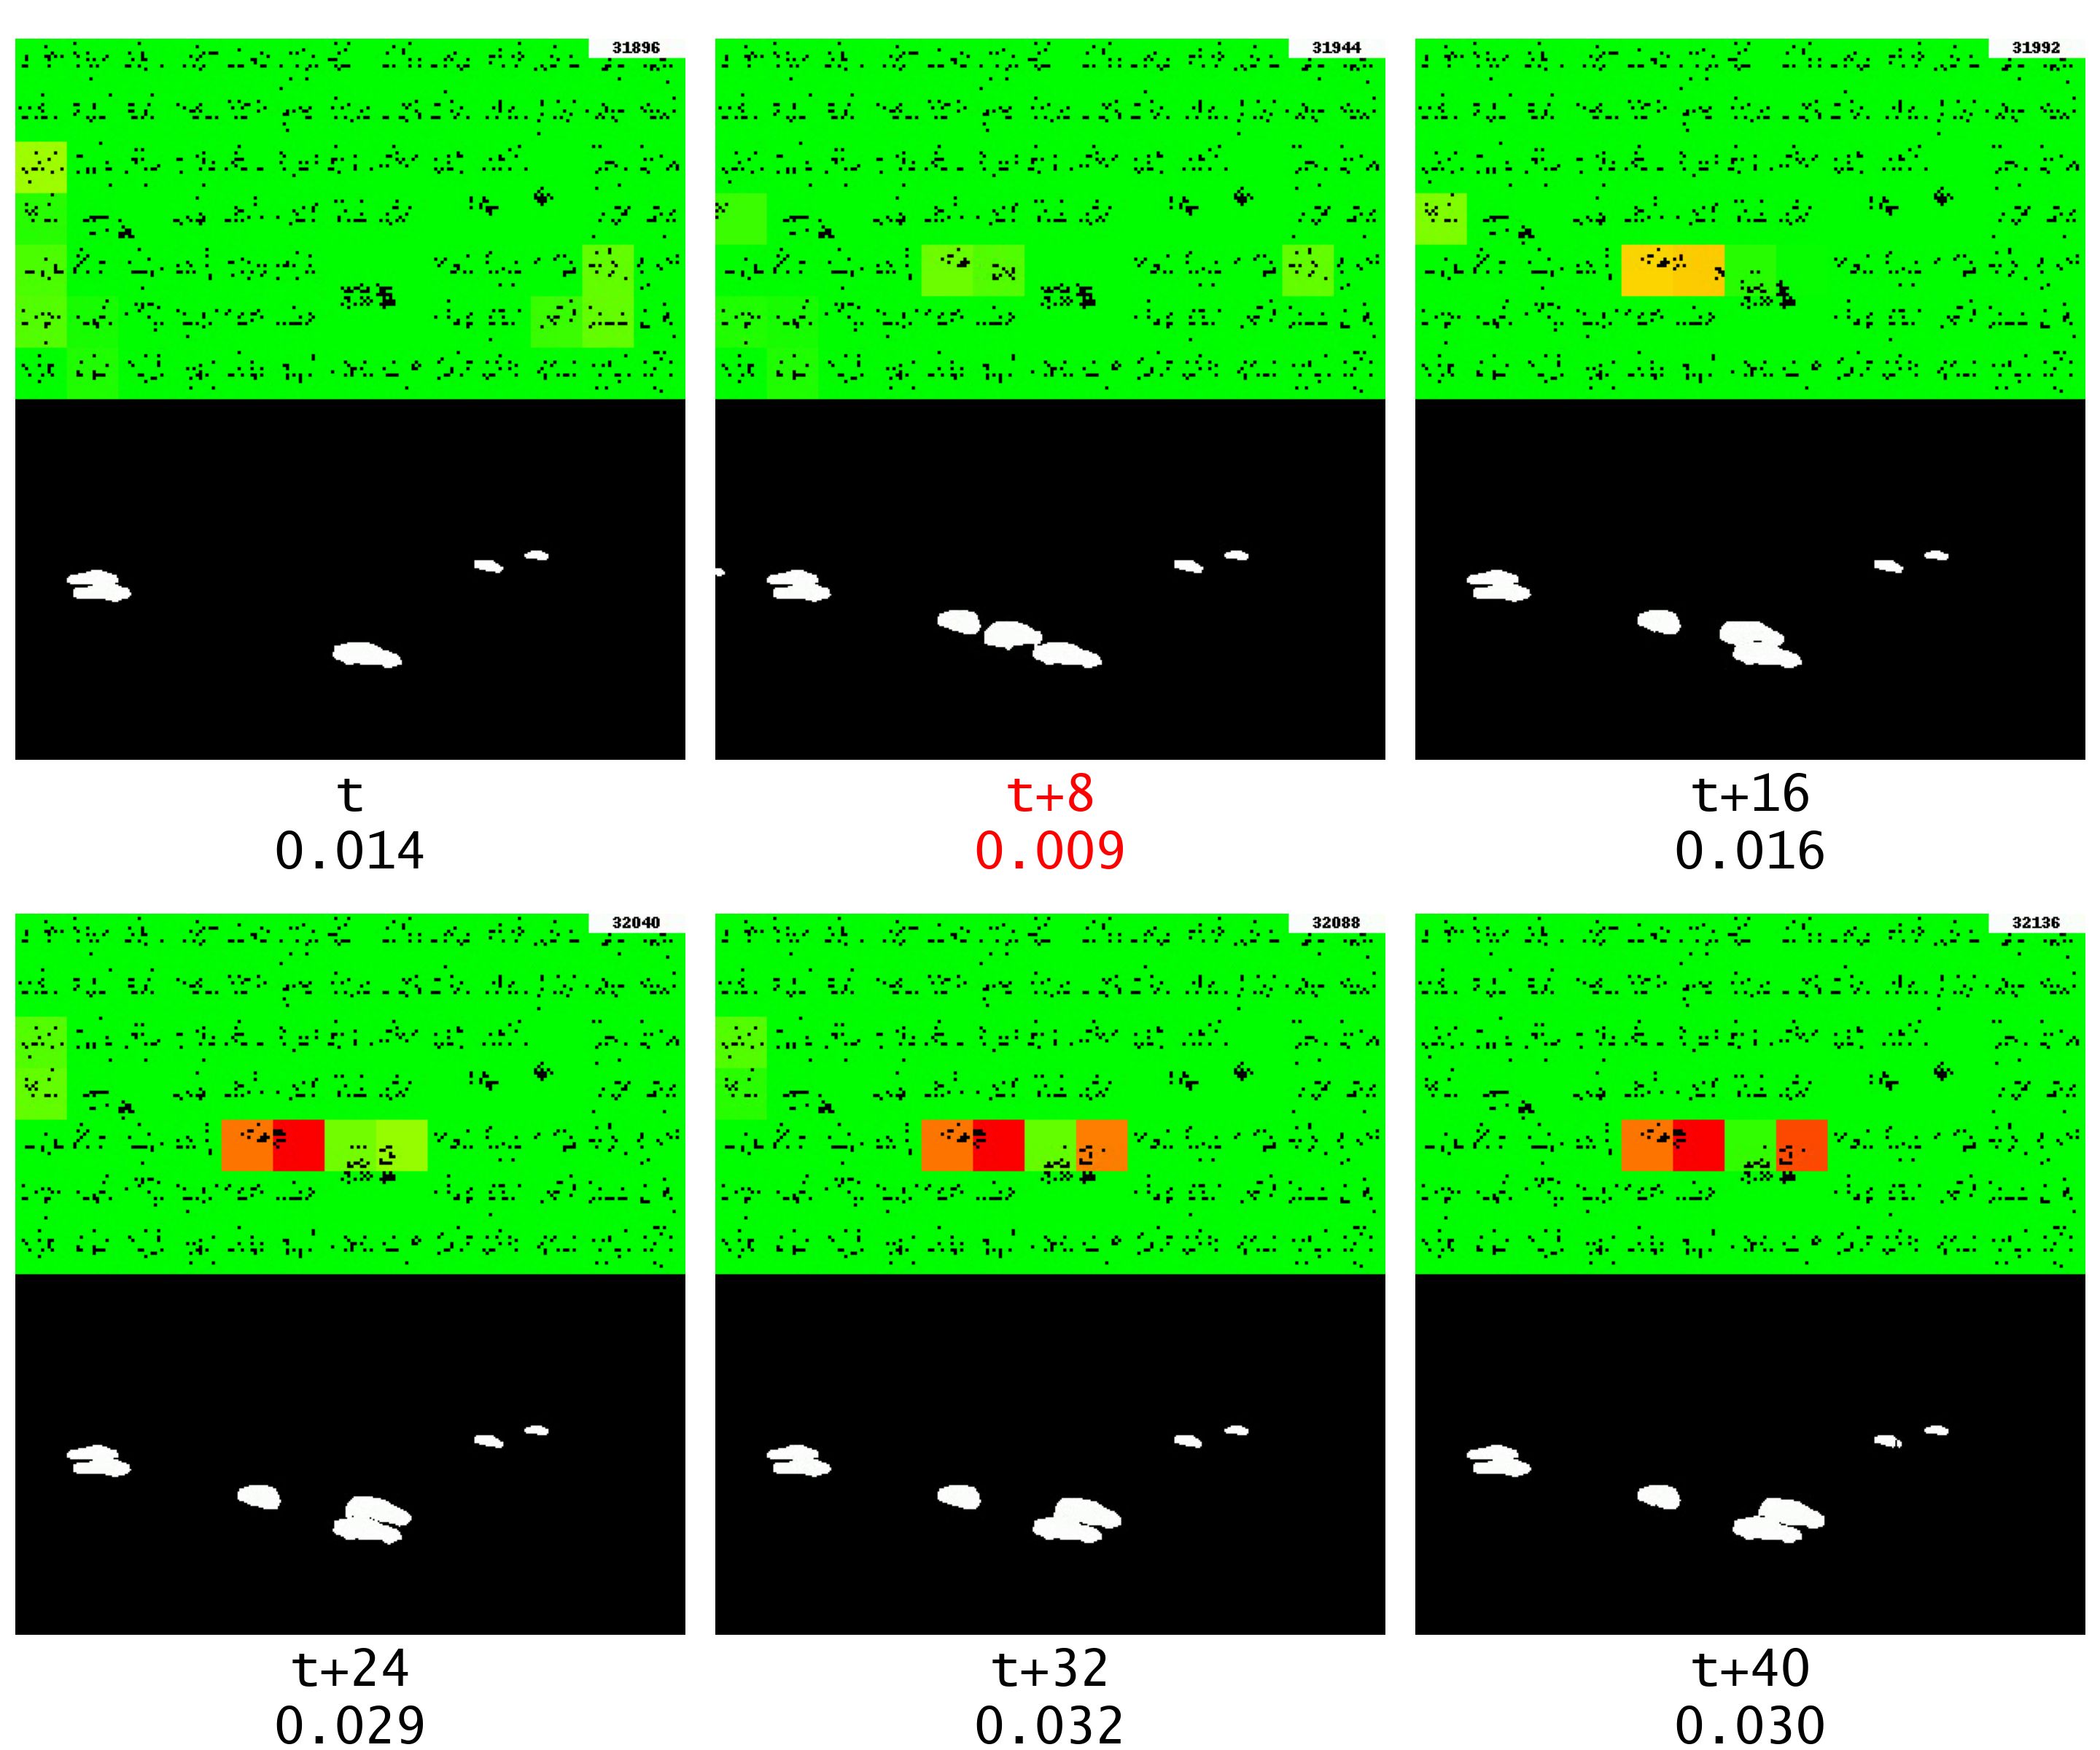
\includegraphics[width=\textwidth]{resources/experiments/surveillance/surveillance_anomaly_1.png}
    \caption[Segment Anomaly]{The first segment anomaly, which is marked with red text,  and the corresponding changes detected by Grid HTM.}
    \label{fig:surveillance_segment}
\end{figure}
Here it is observed that Grid \gls*{htm} correctly marks the sudden change of cars when the current segment ends and a new segment begins.
\subsubsection{Road}
In the original video, there is a road on which cars regularly drive. By observing the visual output, it becomes evident that after some time, Grid \gls*{htm} has mostly learned that behavior and does not report those moving cars as anomalies. This is shown in \autoref{fig:surveillance_road_1}.
\begin{figure}[H]
    \centering
    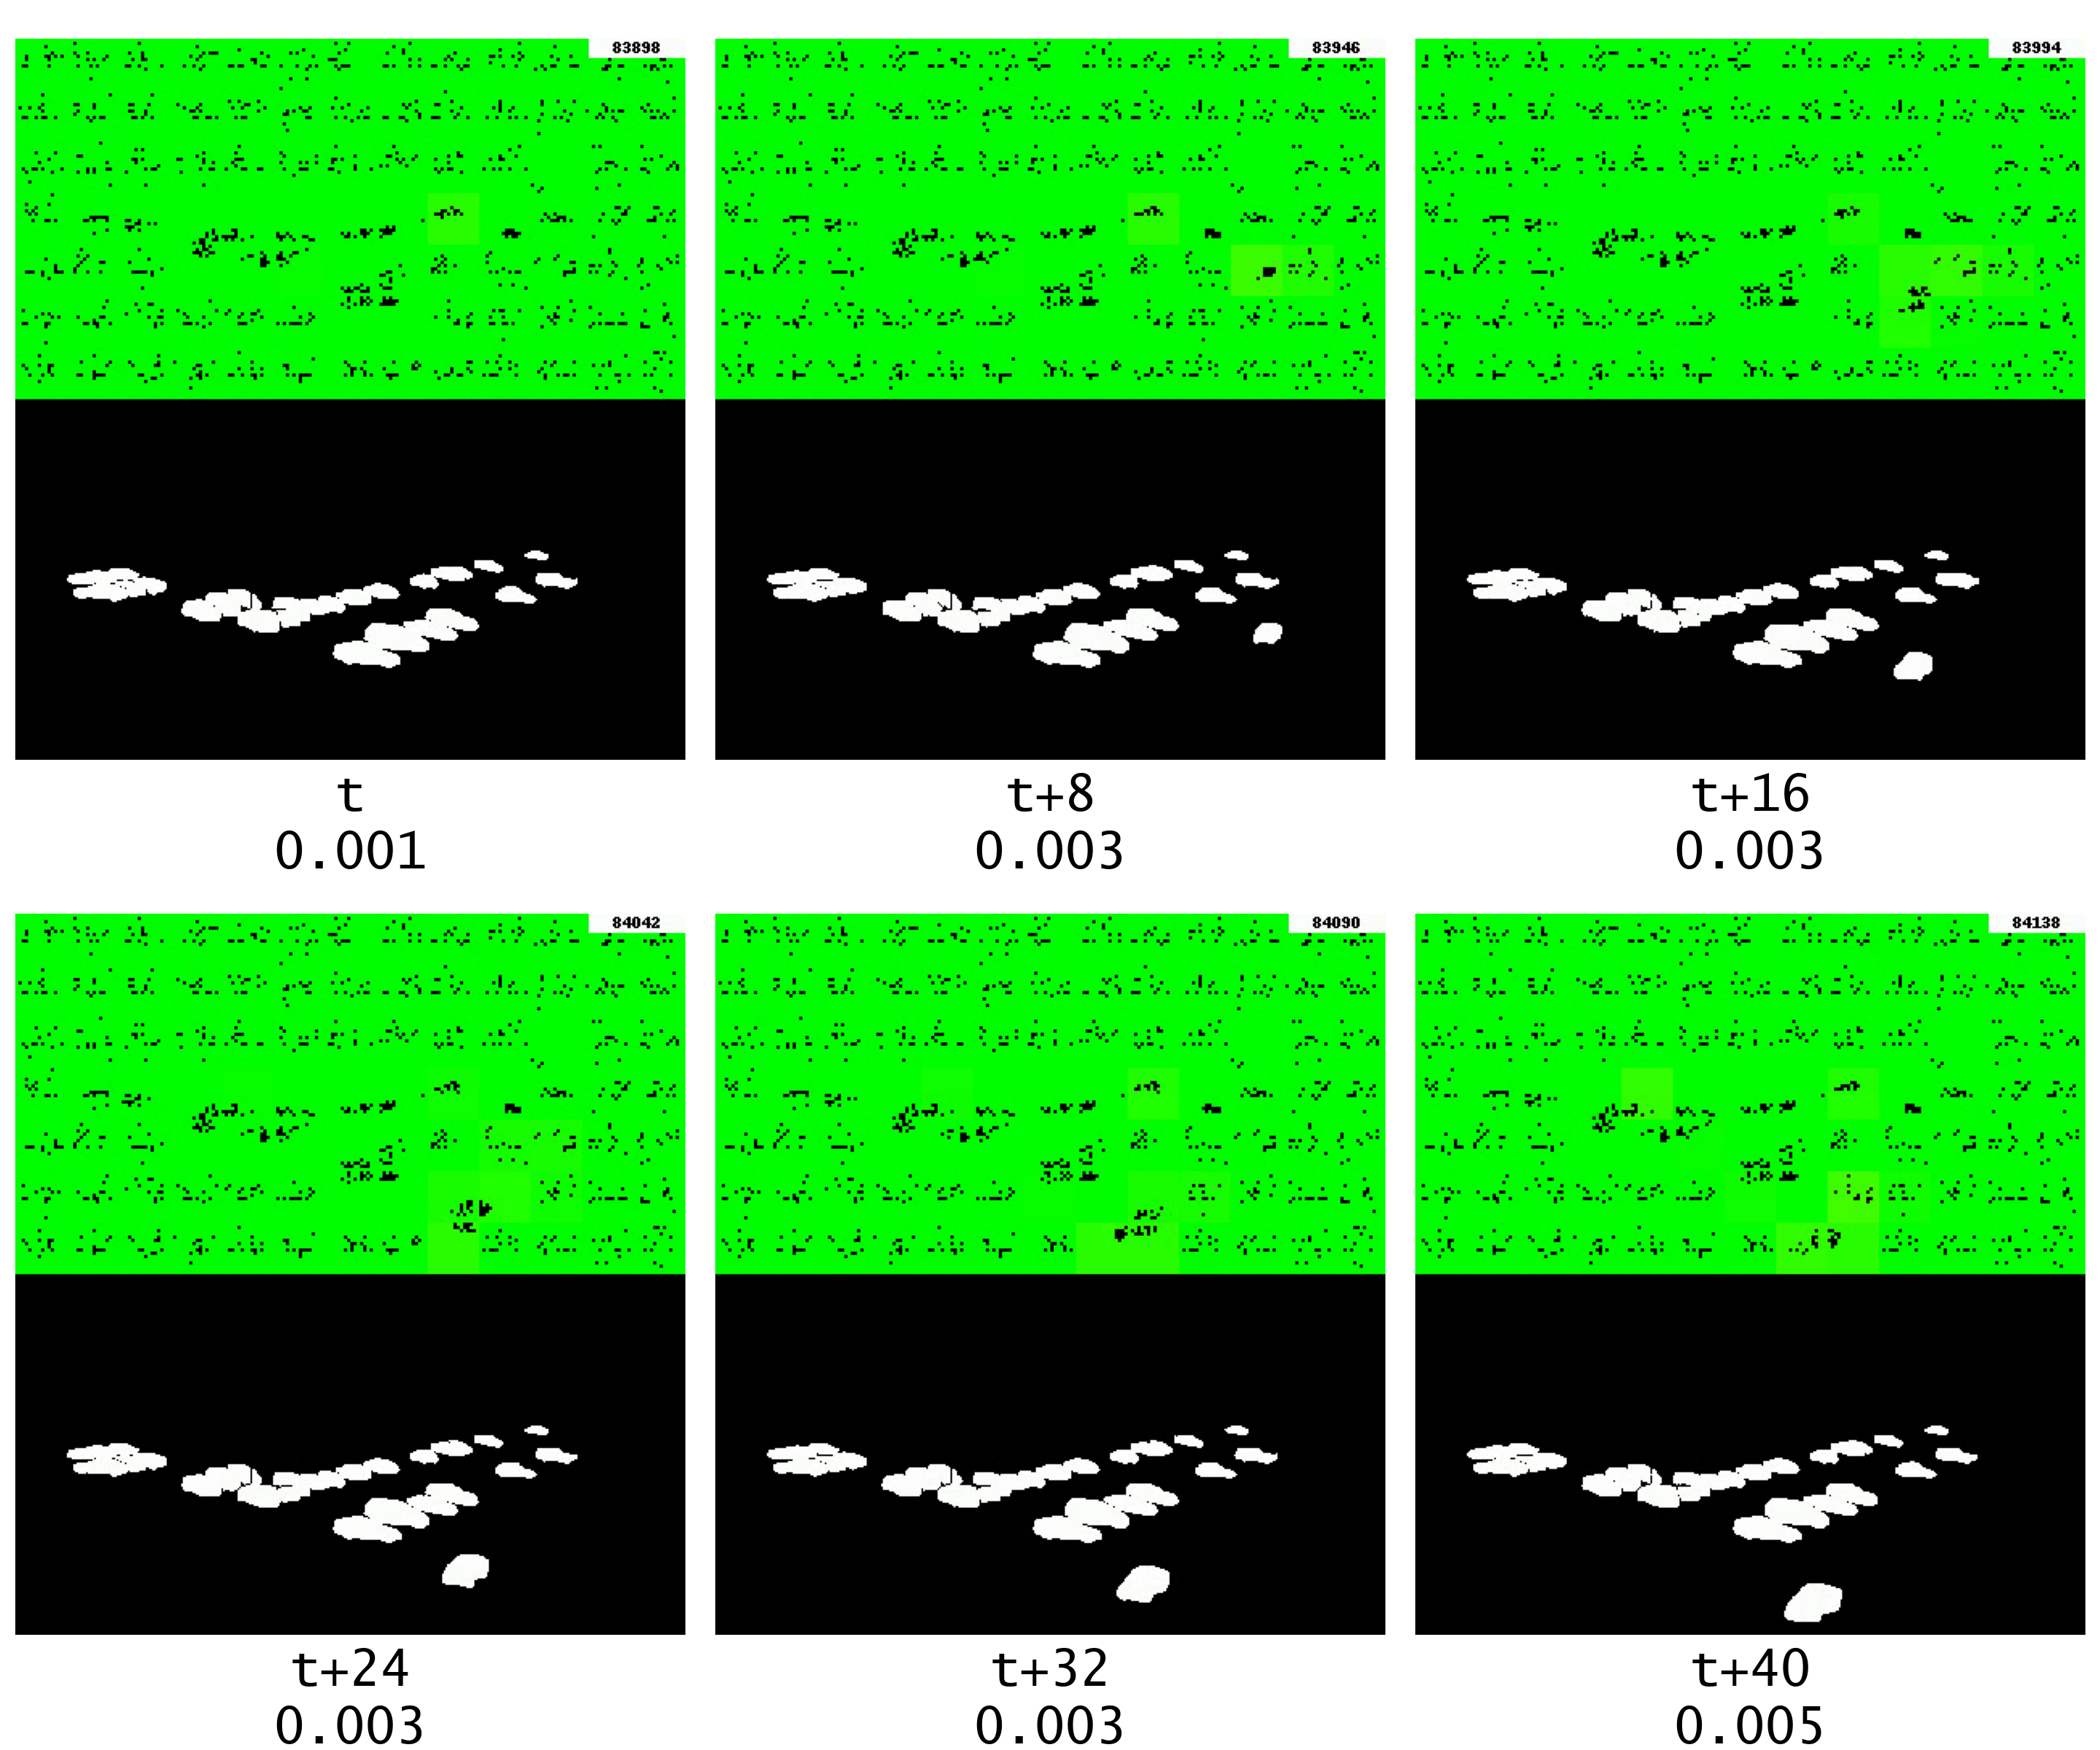
\includegraphics[width=\textwidth]{resources/experiments/surveillance/surveillance_road_1.png}
    \caption[Car Driving Along Main Road]{Visual output during when a car is driving along the main road.}
    \label{fig:surveillance_road_1}
\end{figure}
\subsubsection{Frame Repeat}
To prove that Grid \gls*{htm} has learned that cars on the road should be moving, it is possible to look at the visual output during the period when the video is repeating the same frame and observe if the architecture marks the cars standing still on the road as anomalies.
\begin{figure}[H]
    \centering
    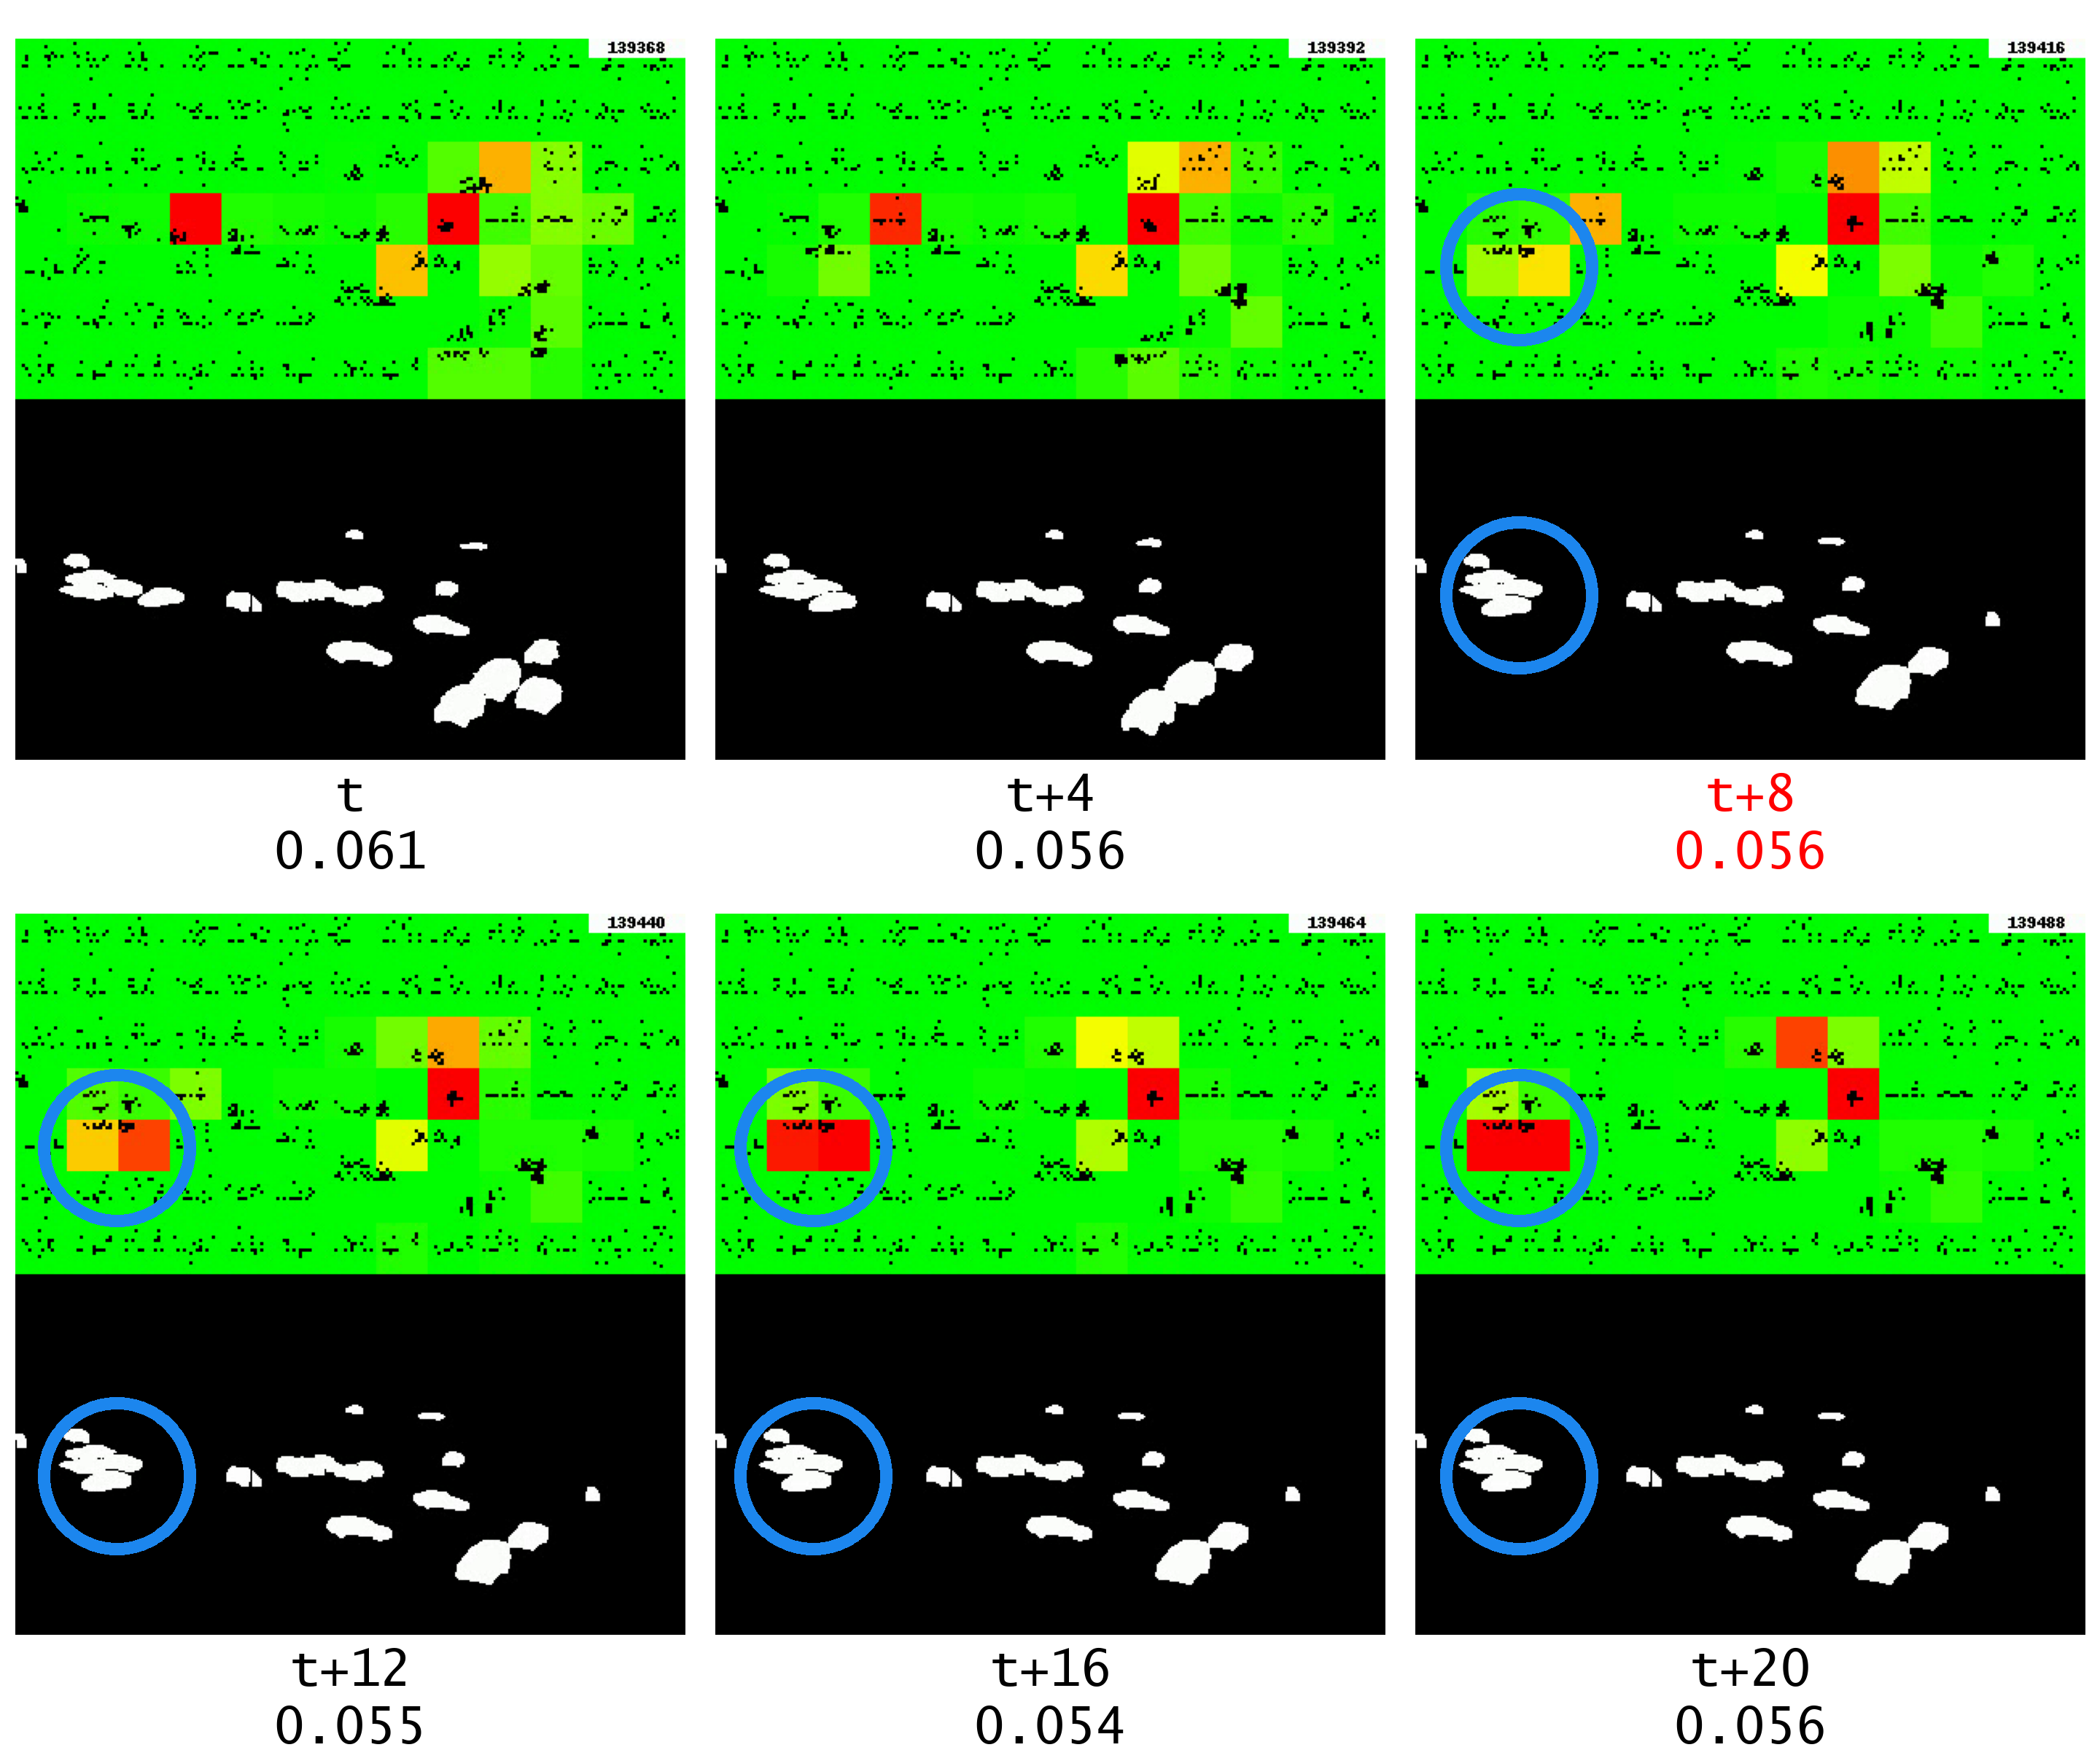
\includegraphics[width=\textwidth]{resources/experiments/surveillance/surveillance_freeze_1.png}
    \caption[Frame Repeat Anomaly]{Anomaly output during the repeating frame, the start of the frame repeat is marked with red text. The blue circle highlights the object of interest.}
    \label{fig:surveillance_freeze_1}
\end{figure}
It can be observed in \autoref{fig:surveillance_freeze_1} that the cars along the main road are not marked as anomalies, but this could be attributed to the fact that there is a crossing there and that cars periodically have to stop at that point to let pedestrians cross.
\par
On the other hand, when looking at the anomaly marked with a blue circle, the car on the road in the parking lot is marked as an anomaly that increases in severity as the time goes on during the frame repeat. The reason why that car causes an anomaly is because, unlike the cars on the main road, a car is rarely observed as standing still at that position.
\par
To prove that the anomaly was actually directly caused by the repeating frame, and not just due to repeating the anomaly in time, it should be compared to the anomaly output if there was no repeating frame.
\begin{figure}[H]
    \centering
    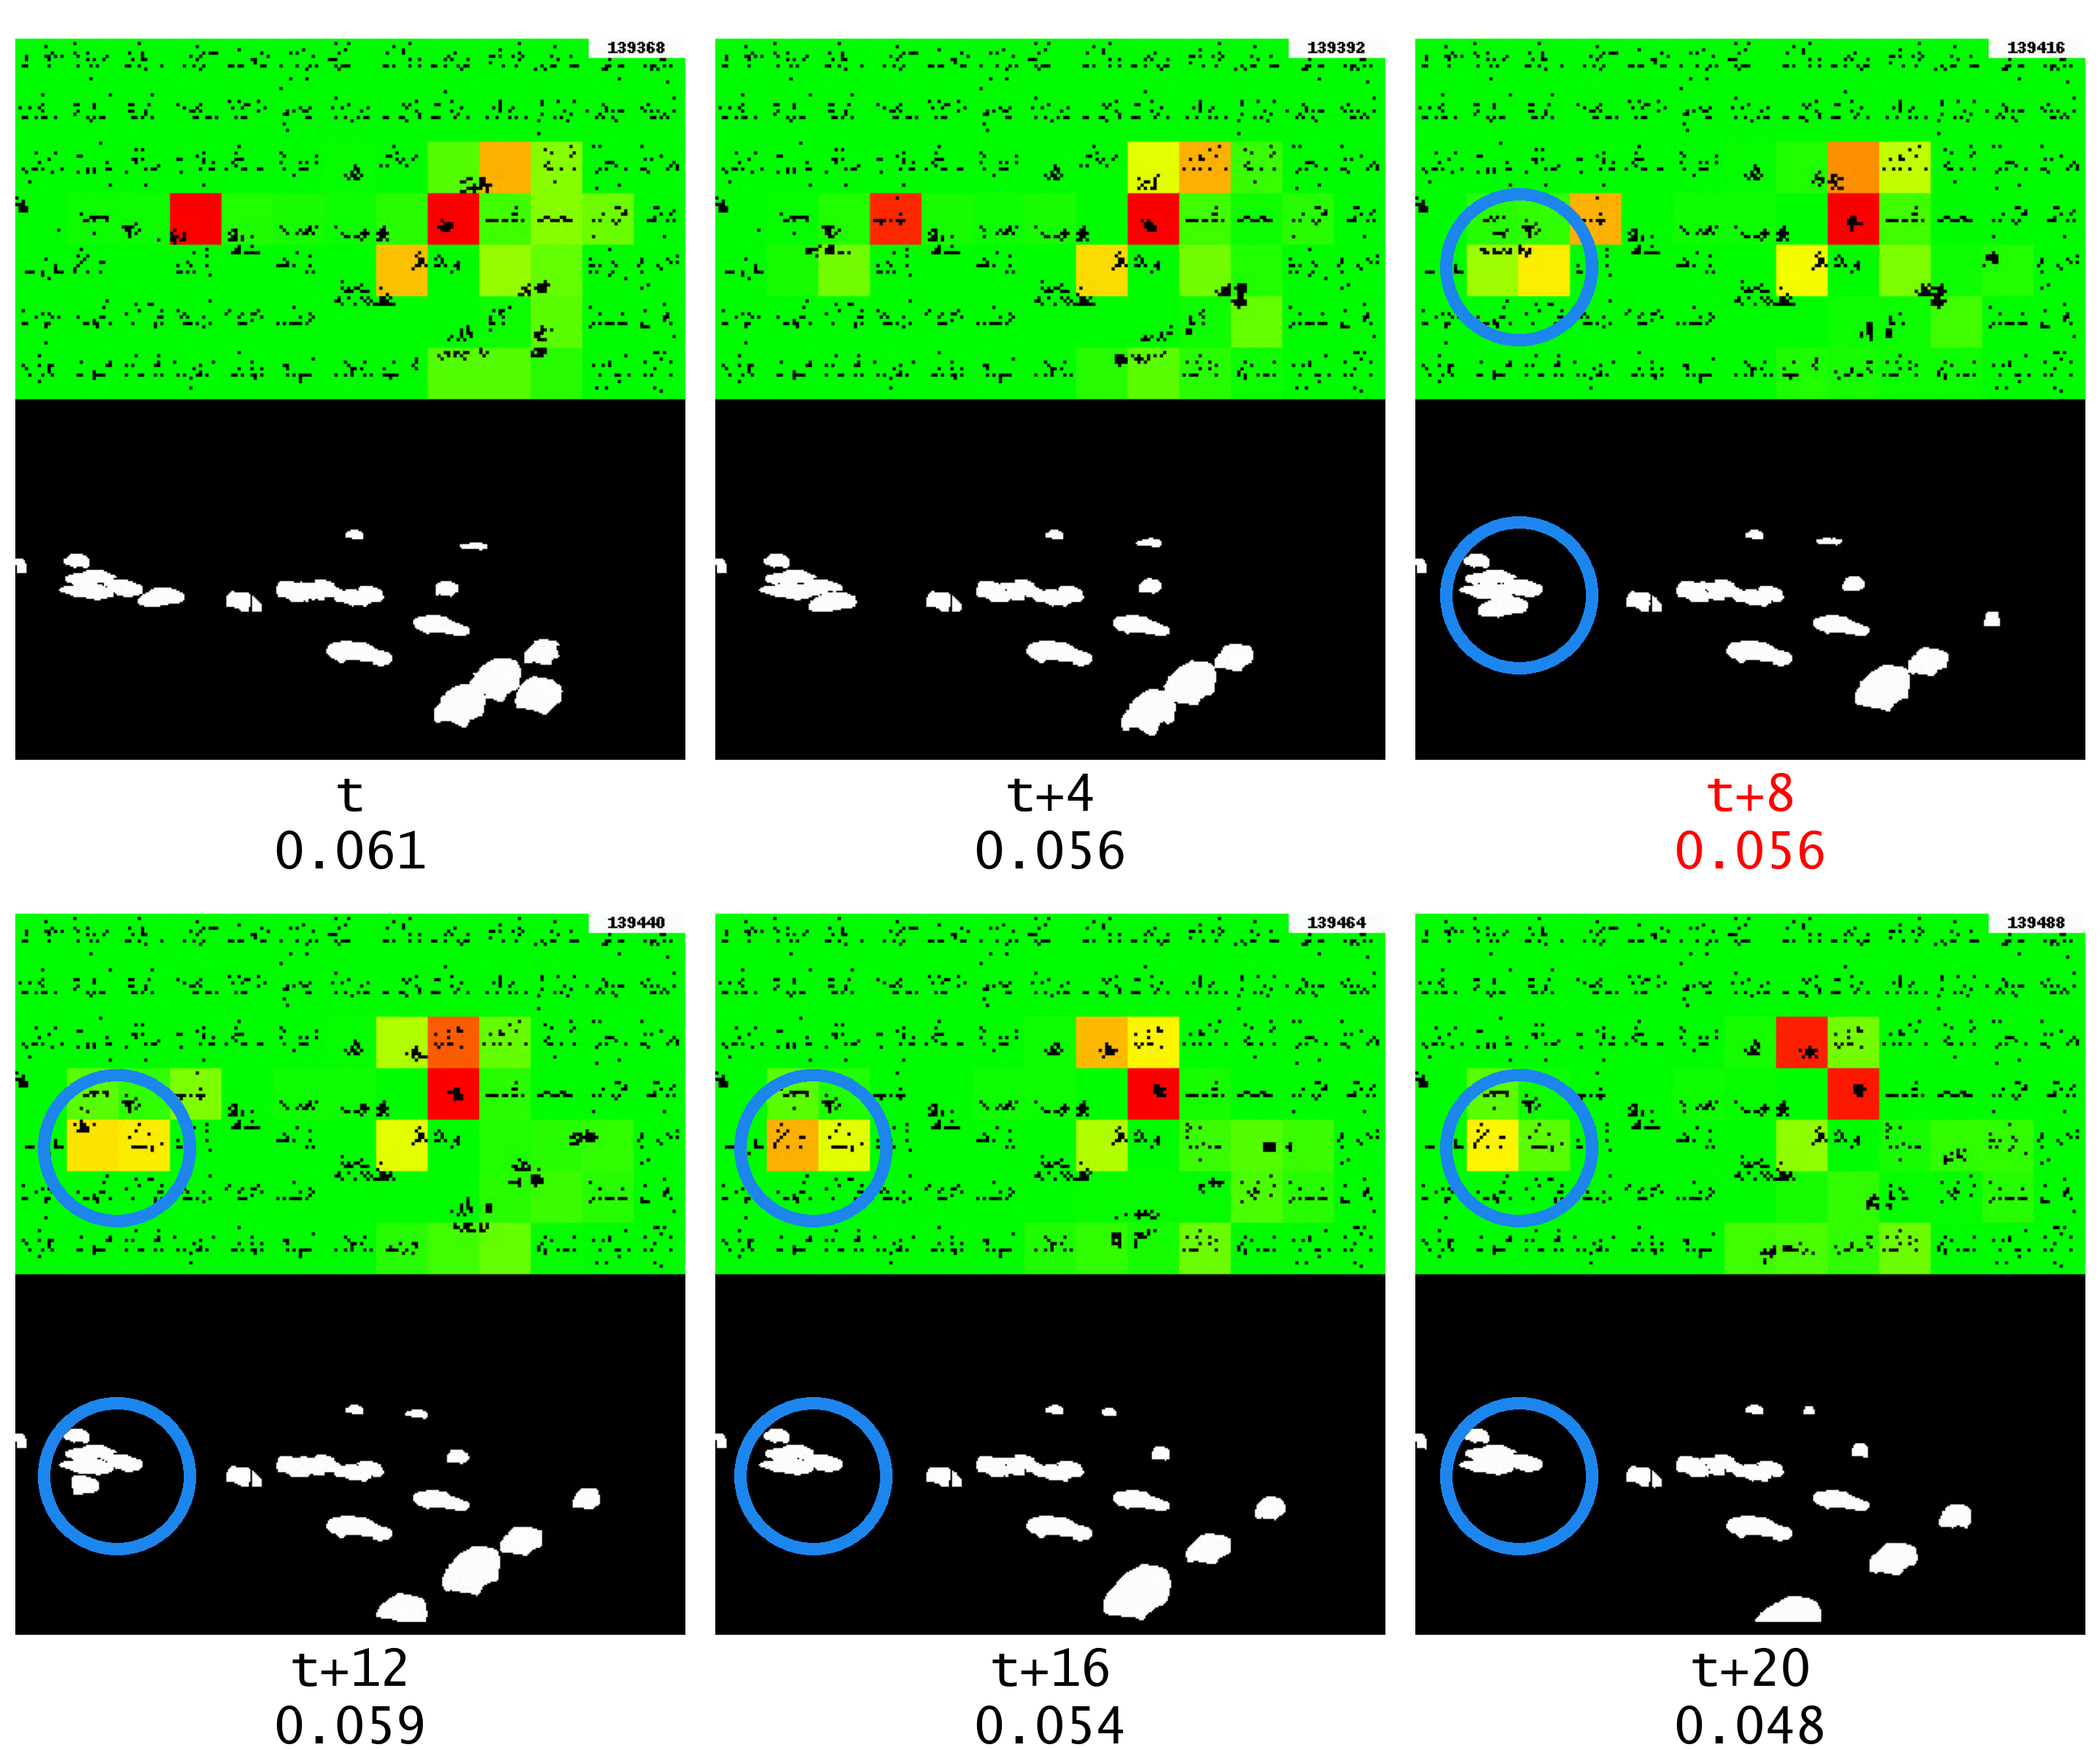
\includegraphics[width=\textwidth]{resources/experiments/surveillance/surveillance_freeze_no_freeze.png}
    \caption[No Frame Repeat Anomaly]{Anomaly output when there is no frame repeating, where it should have repeated is marked in red. The blue circle highlights the object of interest.}
    \label{fig:surveillance_freeze_no_freeze}
\end{figure}
It can be observed in \autoref{fig:surveillance_freeze_no_freeze} that the anomaly output is minor compared to when there was a repeating frame, proving that the anomaly was indeed a product of the repeating frame and that Grid \gls*{htm} was able to learn how objects should be moving in time.
\par
Finally, it is interesting to look at how Grid \gls*{htm} handles the repeating frames without multistep temporal patterns, which is shown in \autoref{fig:surveillance_freeze_no_mtp}.
\begin{figure}[H]
    \centering
    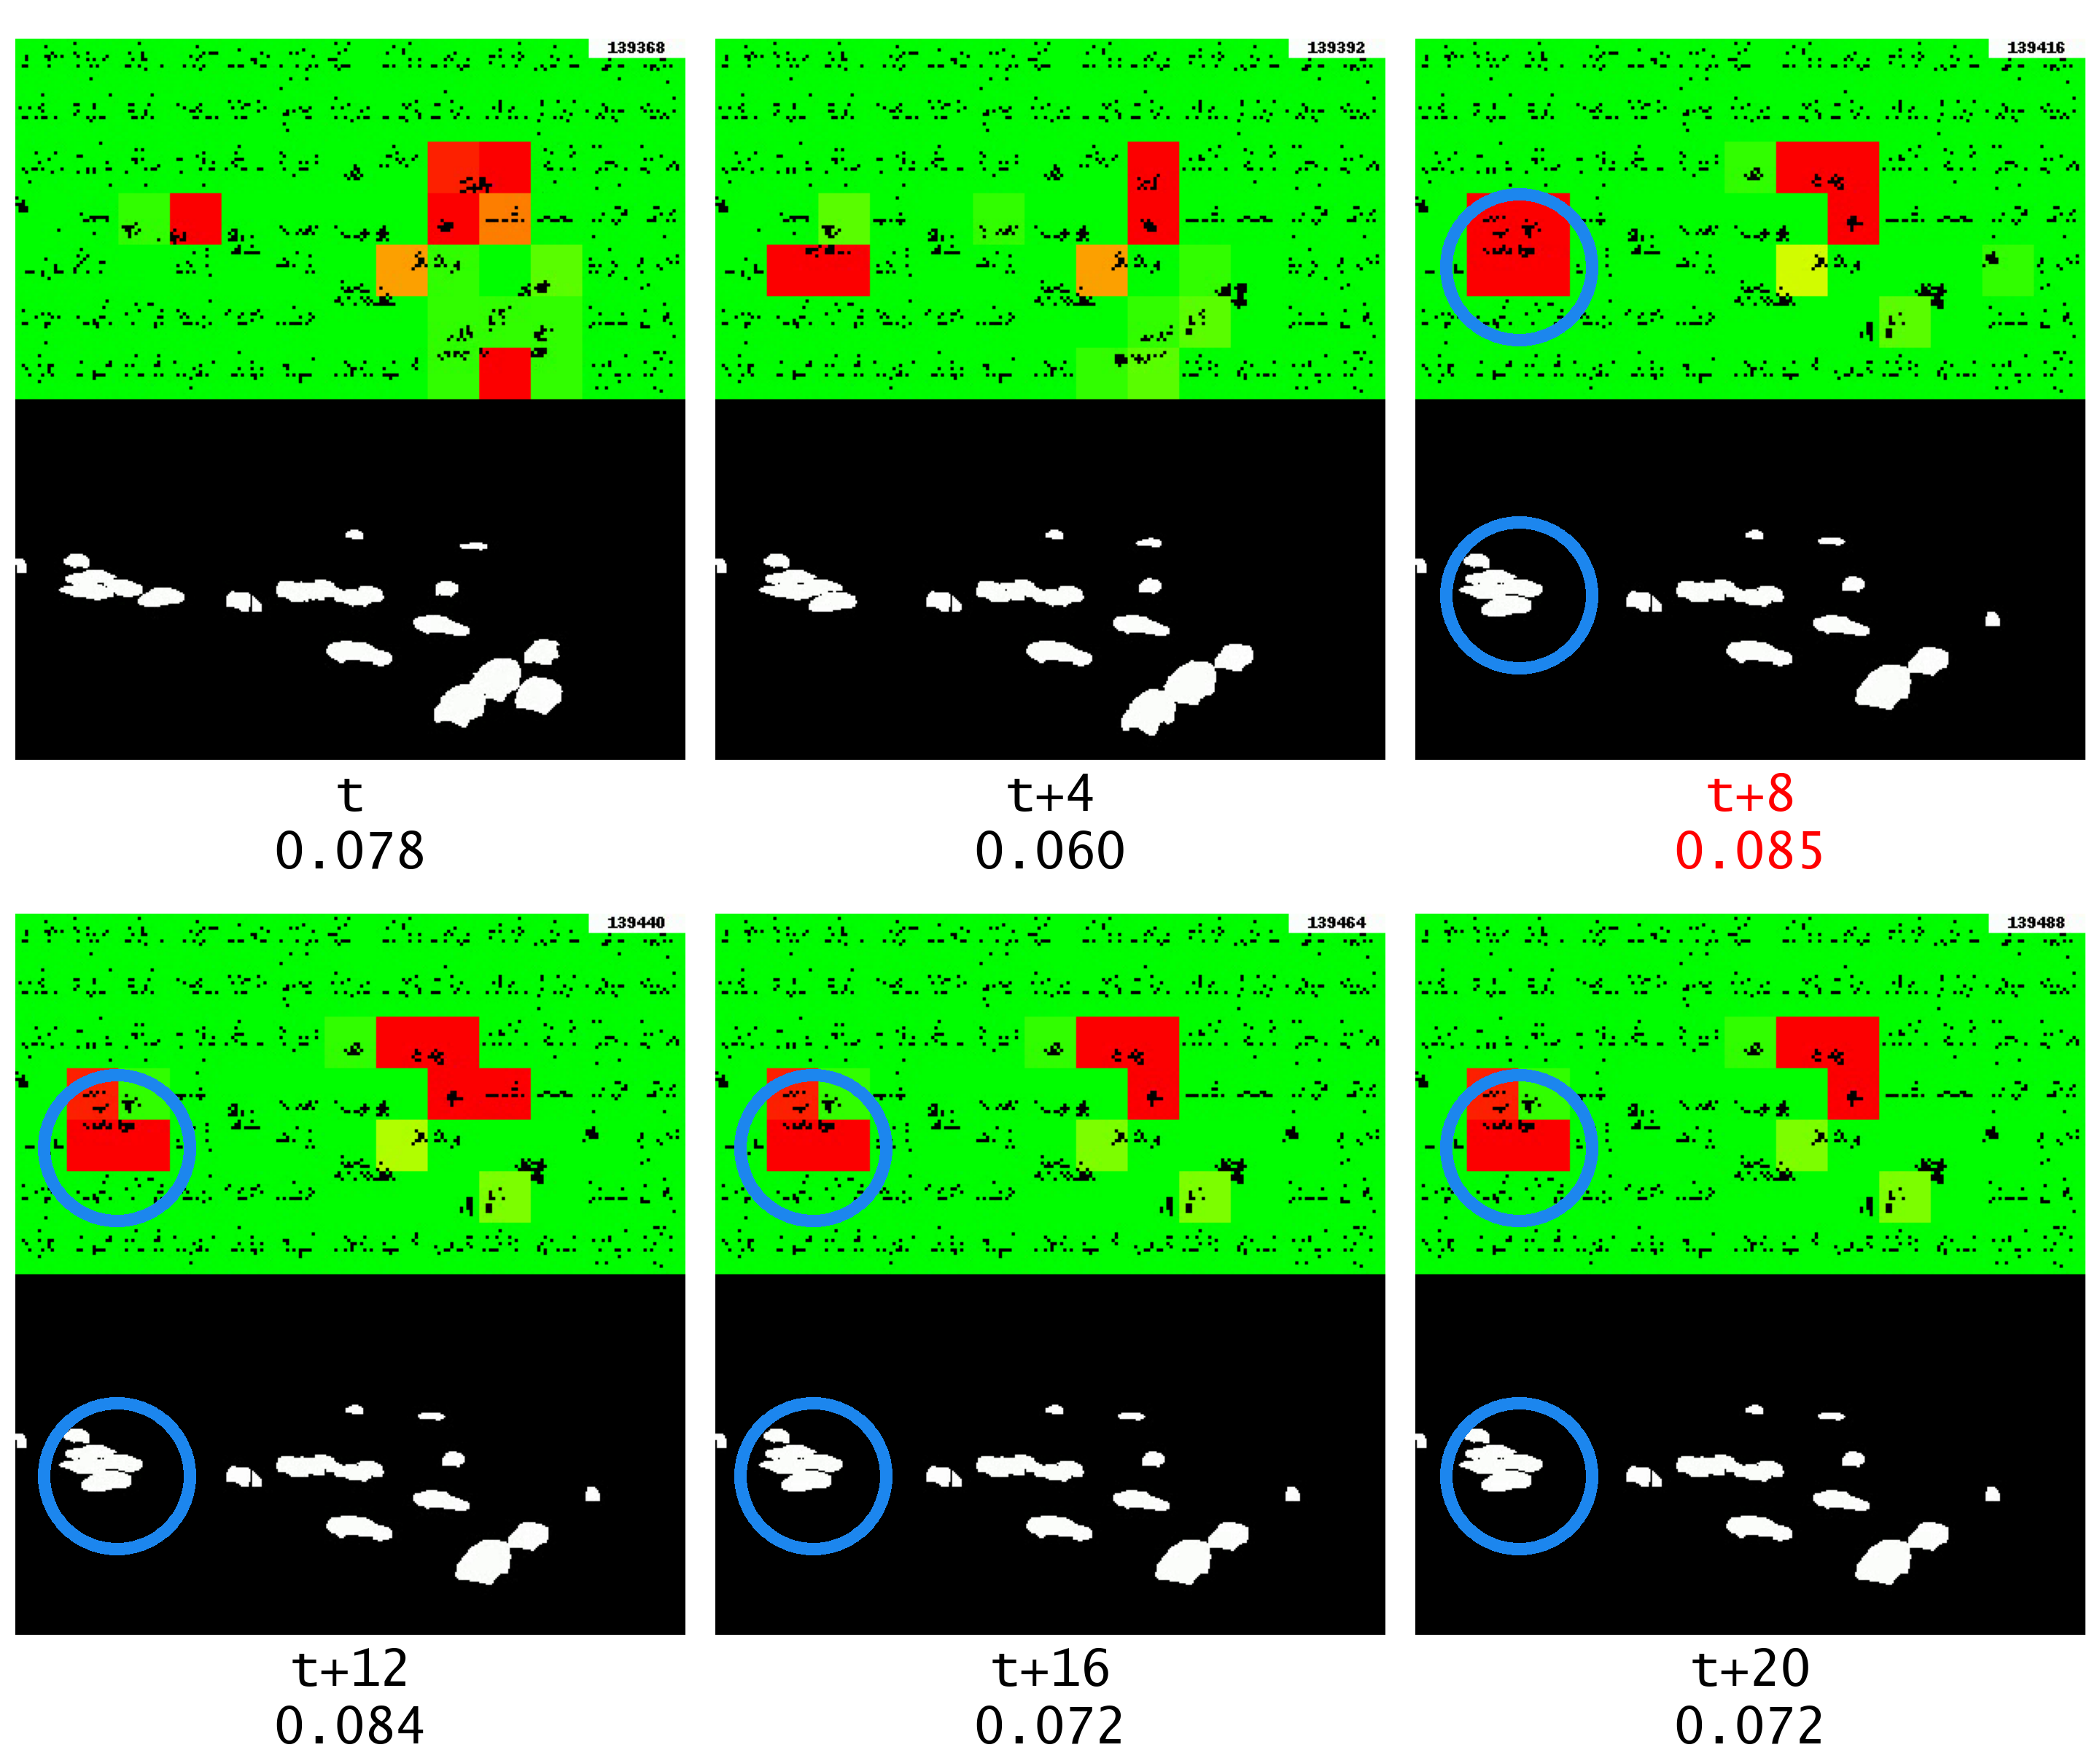
\includegraphics[width=\textwidth]{resources/experiments/surveillance/surveillance_freeze_no_mtp.png}
    \caption[Frame Repeat No Multistep Temporal Pattern Anomaly]{Anomaly output during the repeating frame, the start of the frame repeat is marked with red text. The blue circle highlights the object of interest. This time without multistep temporal patterns.}
    \label{fig:surveillance_freeze_no_mtp}
\end{figure}
Unfortunately, simply disabling multistep temporal patterns without adjusting the other \gls*{tm} parameters causes the same car to be marked as an anomaly before and during the frame repeat. In fact, as mentioned in \autoref{sec:multistep_temporal_patterns}, disabling multistep temporal patterns causes Grid \gls*{htm} to be less noise tolerant which causes a lot more anomalies to be wrongly detected. This is evident in \autoref{fig:surveillance_freeze_no_mtp}, where a higher amount of severe anomalies can be observed compared to previous examples. This also highlights how sensitive \gls*{htm} can be regarding parameters.
\subsubsection{Points of Interest}
Finally, it is interesting to look the various anomaly score spikes and observe in the visual output what caused them. The points of interest to be explored are marked in \autoref{fig:surveillance_poi}
\begin{figure}[H]
    \centering
    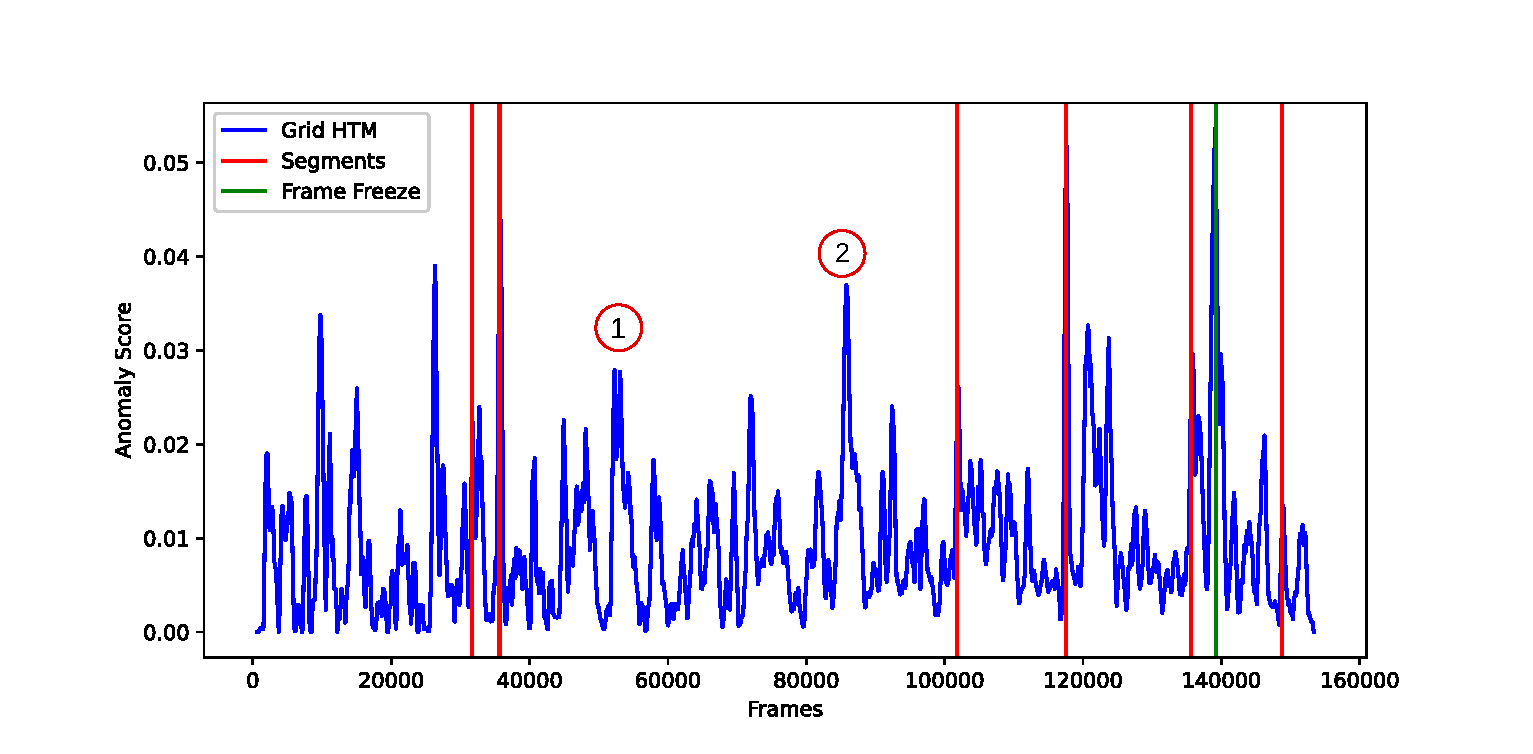
\includegraphics[width=\textwidth]{resources/experiments/surveillance/surveillance_result_poi.eps}
    \caption[Points of Interest]{Points of interests in the anomaly score output.}
    \label{fig:surveillance_poi}
\end{figure}
The first point of interest, which can be seen in \autoref{fig:surveillance_poi_1}, showcases the weakness of the aggregation function.
\begin{figure}[H]
    \centering
    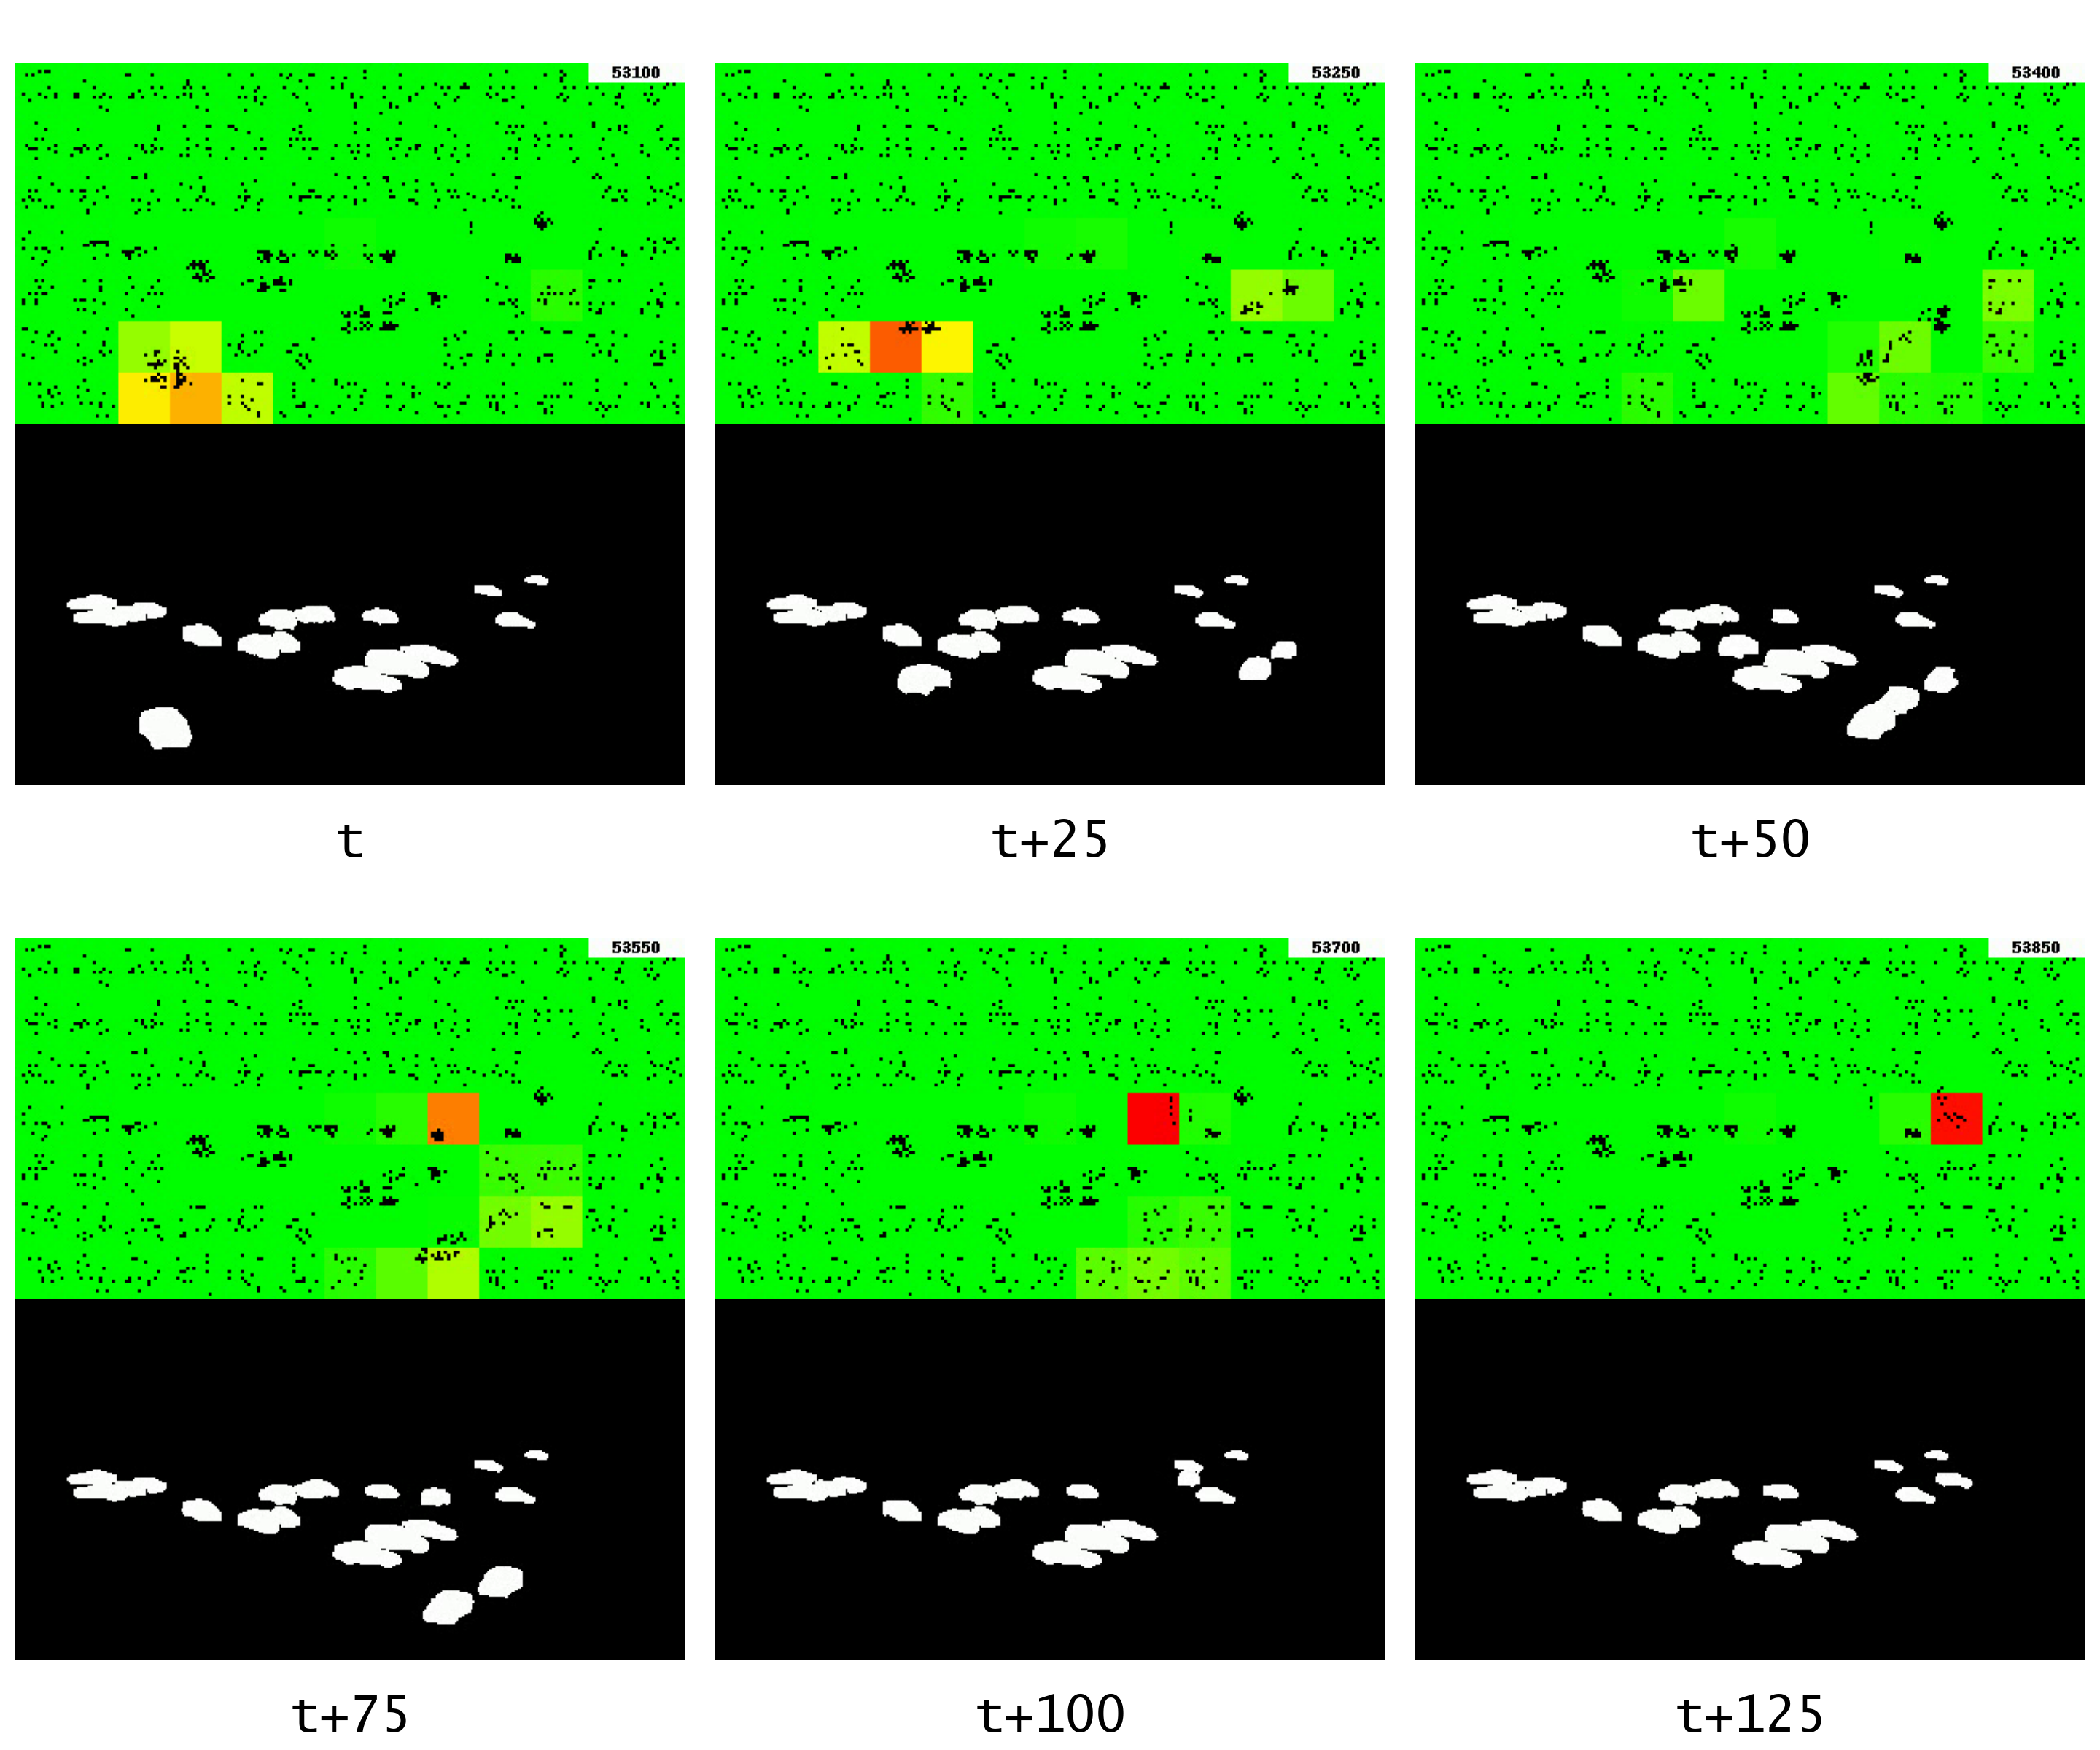
\includegraphics[width=\textwidth]{resources/experiments/surveillance/surveillance_poi_1.png}
    \caption[First POI]{Visual output of the first point of interest.}
    \label{fig:surveillance_poi_1}
\end{figure}
It can be seen that the anomaly score output, which is shown at the very bottom of each image, can be attributed to two occurrences. The first occurrence is a physically big but low severity anomaly. The second occurrence is a physically small but high severity anomaly. Despite the two different anomalies, the anomaly score output is similar for both occurrences.
\par
The second point of interest, which can be seen in \autoref{fig:surveillance_poi_2}, showcases the importance of exposing \gls*{htm} to all possible behaviours that are considered not anomalous, which is one of the complexities mentioned in \autoref{sec:anomaly_detection}.
\begin{figure}[H]
    \centering
    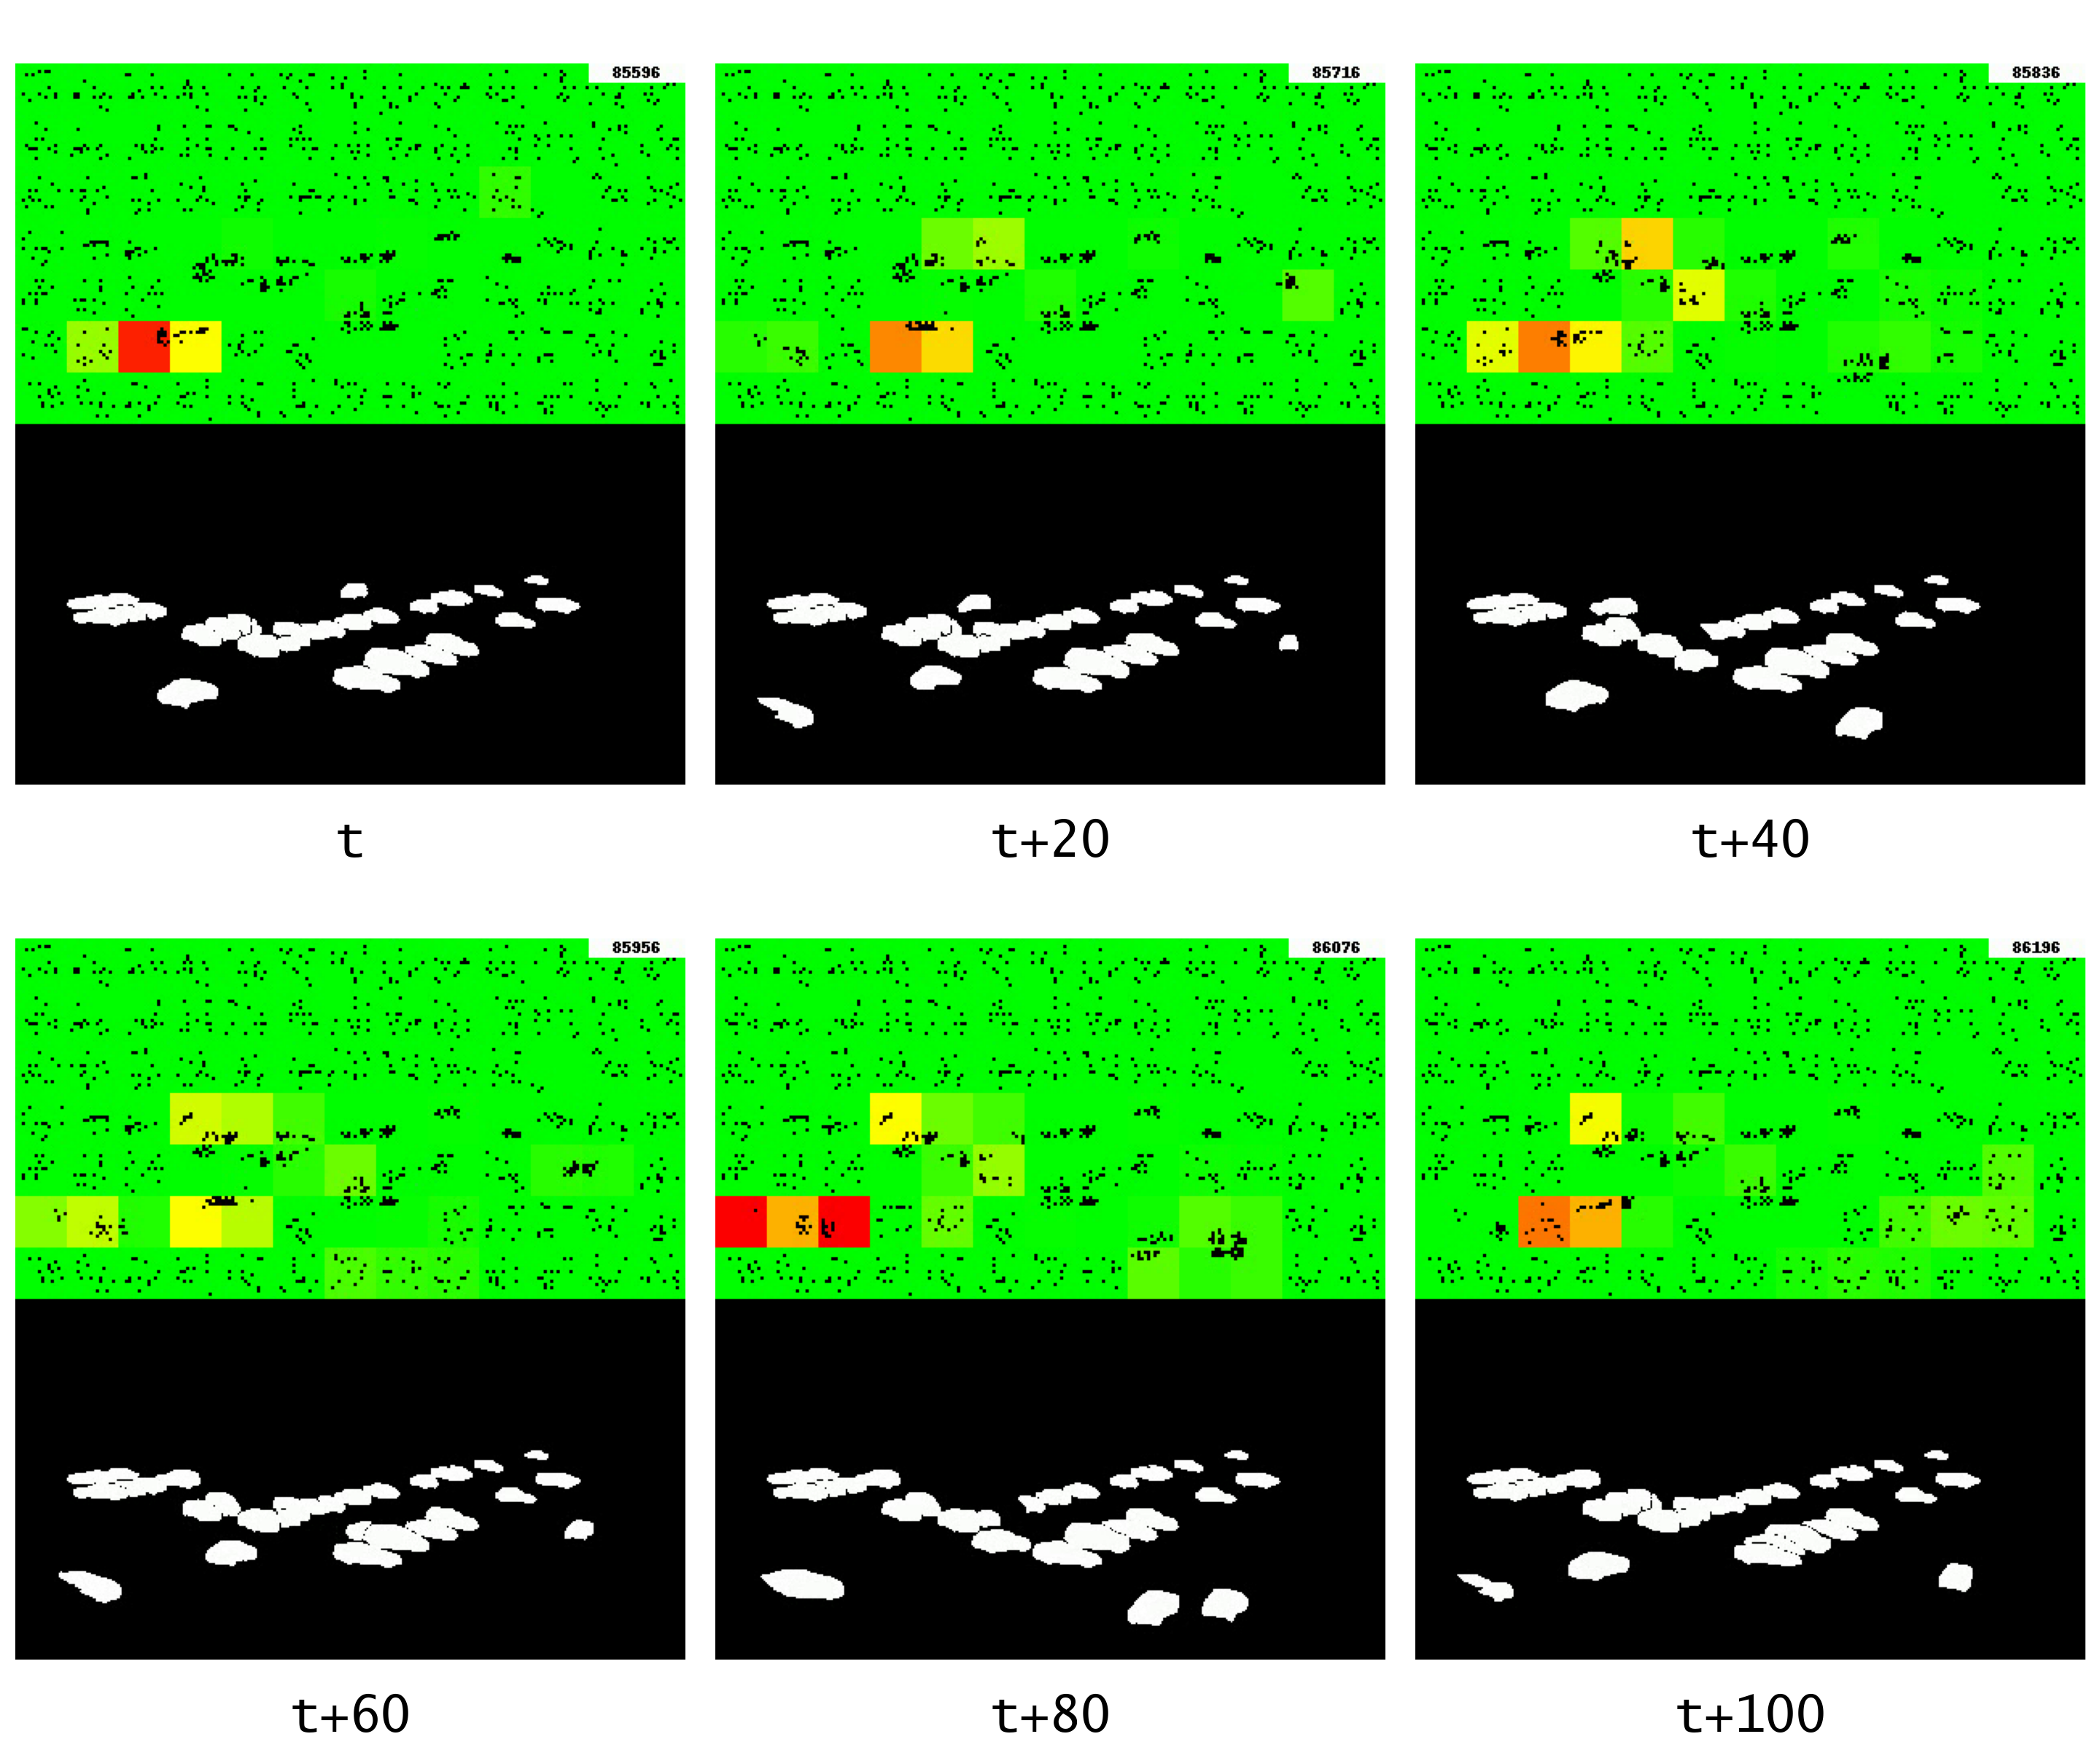
\includegraphics[width=\textwidth]{resources/experiments/surveillance/surveillance_poi_2.png}
    \caption[Second POI]{Visual output of the second point of interest.}
    \label{fig:surveillance_poi_2}
\end{figure}
It can be observed that there are high anomaly outputs for cars entering the parking lot from the left side of the frame. The high anomaly score is caused by an insufficient amount of previous observations of that behavior.
\subsection{Parameters}
Final list of parameters for reproducibility. As previously mentioned, a moving average ($n=200$) was used to smooth the output graph and make it more readable. The mean was used as the aggregation function due to the complex nature of the data.
\begin{table}[H]
    \centering
    \begin{tabularx}{\linewidth}{@{}XlX@{}}
        \toprule
        \textbf{Parameter} & \textbf{Value} & \textbf{Notes}                                \\
        \midrule
        sp\_grid\_size     & 32, 32         & Size of each grid                             \\
        tm\_grid\_size     & 16, 16         & Size of each \gls*{sp} grid output.           \\
        min\_sparsity      & 10             &                                               \\
        sparsity           & 15             & Expected average sparsity                     \\
        temporal\_size     & 15             & Size of the multistep temporal pattern buffer \\
        \bottomrule
    \end{tabularx}
    \caption{Grid HTM specific parameters}
    \label{tab:surveillance_grid_htm}
\end{table}
\begin{table}[H]
    \centering
    \begin{tabularx}{\linewidth}{@{}XlX@{}}
        \toprule
        \textbf{Parameter} & \textbf{Value} & \textbf{Notes}                    \\
        \midrule
        inputDimensions    & sp\_grid\_size &                                   \\
        columnDimensions   & tm\_grid\_size &                                   \\
        potentialPct       & 0.2            &                                   \\
        potentialRadius    & 5              &                                   \\
        localAreaDensity   & 0.05           &                                   \\
        globalInhibition   & True           & Set to False to enable topology   \\
        wrapAround         & False          &                                   \\
        synPermActiveInc   & 0.01           &                                   \\
        synPermInactiveDec & 0.00001                                            \\
        stimulusThreshold  & 3              &                                   \\
        boostStrength      & 0              & Causes instability in empty cells \\
        \bottomrule
    \end{tabularx}
    \caption{SP Parameters}
    \label{tab:surveillance_sp}
\end{table}
\begin{table}[H]
    \centering
    \begin{tabularx}{\linewidth}{@{}XlX@{}}
        \toprule
        \textbf{Parameter}        & \textbf{Value} & \textbf{Notes}        \\
        \midrule
        columnDimensions          & tm\_grid\_size & Same as the \gls*{sp} \\
        predictedSegmentDecrement & 0.001          &                       \\
        permanenceIncrement       & 0.01           &                       \\
        permanenceDecrement       & 0.001          &                       \\
        minThreshold              & 10             &                       \\
        activationThreshold       & 10             &                       \\
        cellsPerColumn            & 32             &                       \\
        \bottomrule
    \end{tabularx}
    \caption{TM Parameters}
    \label{tab:surveillance_tm}
\end{table}
\subsection{Experiment Summary}
This experiment showcases the performance of Grid \gls*{htm} on complex data, specifically a surveillance video of a parking lot. The video contains technical anomalies in the form of segments, and also a synthetic anomaly which is a period of repeating frames. Semantic segmentation was performed in order to extract the cars in the frame into an SDR.
\par
The results show that Grid \gls*{htm} has the ability to react when segments begin and end, as well as the ability to detect the repeating frames. It also shows that the anomaly output, with the currently introduced aggregation functions, cannot be used to reliably to threshold anomalies. Instead, one can look at the visual output of Grid HTM. The visual output shows that Grid \gls*{htm} is able to detect the change in objects when a segment change occurs.
\par
Results also show that Grid \gls*{htm} learns common patterns such as cars driving on the main road, and does not report that behavior as anomalous. It is also shown that Grid \gls*{htm} can correctly detect the repeating frames, and marks anomalous cars during the repeating frames with an increasing severity. Finally, a couple of points of interests are shown that highlight the weakness of the aggregation function and the importance of exposing \gls*{htm} to all possible behaviors not considered anomalous.
\clearpage
\section{Sperm Experiment}
As seen in the surveillance experiment, it seems Grid \gls*{htm} can detect when segments begin and end. This experiment will explore this ability in greater detail.
\subsection{Data}
The dataset used is VISEM~\cite{VISEM}, a sperm dataset which consists of videos that are made up of several segments. The sperm cells will be segmented using a rough binary thresholding, as shown in \autoref{fig:sperm_segmentation}.
\begin{figure}[H]
    \centering
    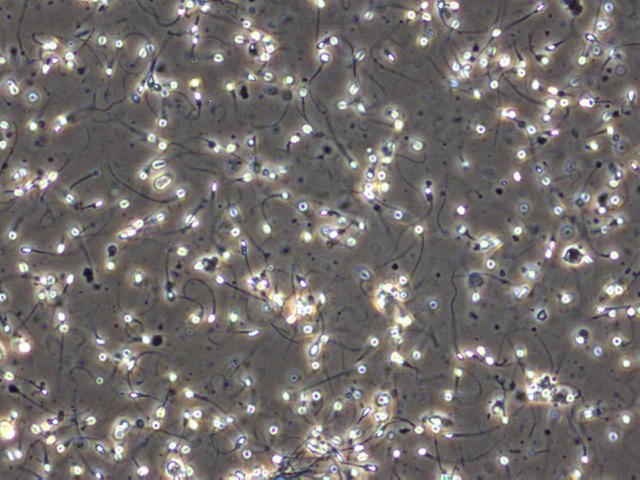
\includegraphics[width=.45\textwidth]{resources/experiments/sperm/sperm_example.png}
    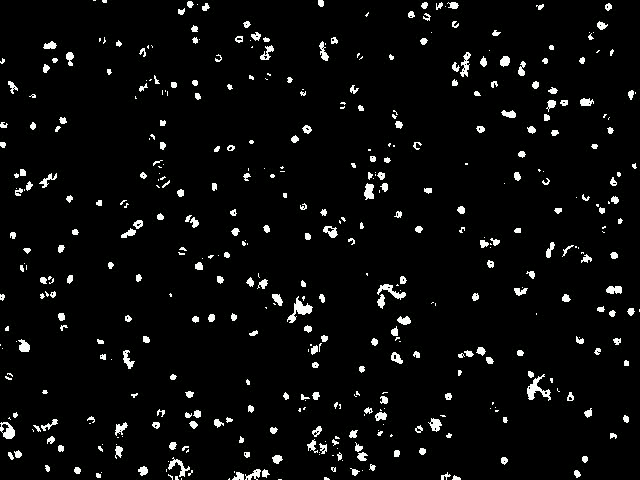
\includegraphics[width=.45\textwidth]{resources/experiments/sperm/sperm_seg_example.png}
    \caption[Sperm Example Frame]{Example frame from a sperm video (left) and its corresponding segmentation (right).}
    \label{fig:sperm_segmentation}
\end{figure}
It is important to note that the data itself is noisy, and that it is not possible for Grid \gls*{htm} to learn any meaningful pattern. The individual videos are also relatively short, which makes it even harder to learn any meaningful patterns.
\subsection{Benchmark}
To ensure that \gls*{htm} does not just react to the sudden change in pixels but does something more, the L1 error will be used as a benchmark to compare against:
\begin{align*}
    E_t=\sum|F_t-F_{t-1}|
\end{align*}
Where $F_t$ denotes a segmented frame at time step $t$. The L2 error could also have been used, but it would not matter since this experiment will be comparing relative values.
\subsection{Results}
As seen in \autoref{fig:sperm_results1}, Grid \gls*{htm} is able to outperform the L1 error benchmark. This can be deduced from the more prominent changes in the anomaly score, compared to the L1 error. The reason might be that even though the data is very noisy, there is still something in it which makes Grid \gls*{htm} able to learn something general about the current state. This could for instance be a single cell that is standing still or moving very slowly, which Grid \gls*{htm} anchors itself to and uses it to determine when segments start and end.
\begin{figure}[H]
    \centering
    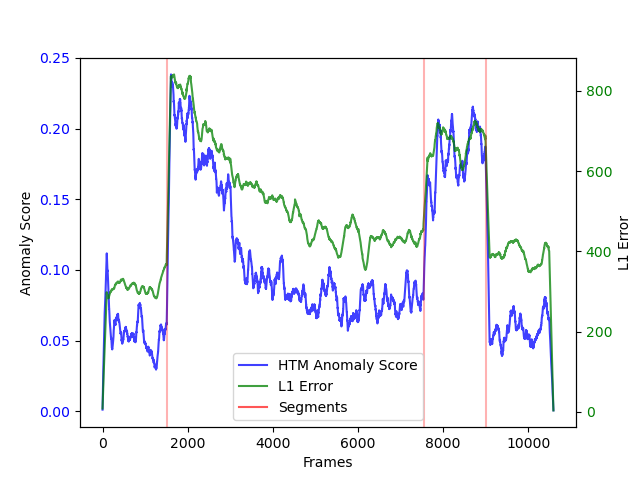
\includegraphics[width=\textwidth]{resources/experiments/sperm/sperm_result1.png}
    \caption[Stationary Video Results]{Results on a stationary sperm video.}
    \label{fig:sperm_results1}
\end{figure}

\par
That being said, the parameters for Grid \gls*{htm} were selected carefully to achieve the results seen in \autoref{fig:sperm_results1}, and are dependent on the contents of the data. Unfortunately, most of the videos in the dataset contain drift (in other words, the video is not stationary), which makes Grid \gls*{htm} useless. This can be observed in \autoref{fig:sperm_results2}, where both Grid \gls*{htm} and the L1 error struggle.
\begin{figure}[H]
    \centering
    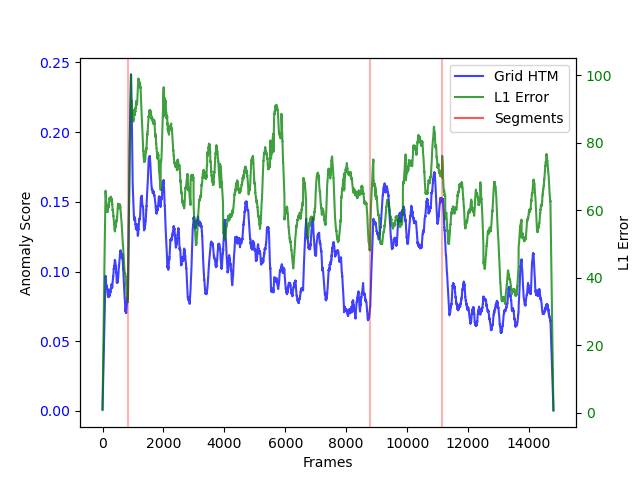
\includegraphics[width=\textwidth]{resources/experiments/sperm/sperm_result2.png}
    \caption[Drifting Video Results]{Results on a sperm video with drift.}
    \label{fig:sperm_results2}
\end{figure}
Just like in the stationary video, the change in the anomaly score is more pronounced, but due to the drift in the video there is a constant high anomaly output which makes it impossible to find a threshold value. That being said, Grid \gls*{htm} still outperforms the L1 score due to the more prominent changes in the anomaly score.
\subsection{Use Cases}
The use case is to be able to use Grid \gls*{htm} to detect segments and then use a separate tool to extract each segment. This could be useful in data processing, or even in streaming media services to automatically know when cuts happen and could aid scene boundary detection systems~\cite{scene_boundary_detection}.
\subsection{Parameters}
The following parameters were used in this experiment. The main difference from the surveillance experiment to note is the temporal size, which has been disabled due to the nonexistent patterns in the data. For the plots, a moving average with window size $n=100$ was used to smooth the lines and reduce noise in the output graph. Because the data is noisy, the mean was used as the aggregation function. For binary thresholding, a pixel value threshold of $k=200$ was used.
\begin{table}[H]
    \centering
    \begin{tabularx}{\linewidth}{@{}XlX@{}}
        \toprule
        \textbf{Parameter} & \textbf{Value} & \textbf{Notes}                                                                    \\
        \midrule
        sp\_grid\_size     & 16, 16         & Size of each grid                                                                 \\
        tm\_grid\_size     & 8, 8           & Size of each \gls*{sp} grid output.                                               \\
        min\_sparsity      & 1              &                                                                                   \\
        sparsity           & 5              &                                                                                   \\
        temporal\_size     & 1              & Size of the multistep temporal pattern buffer, 1 means it is effectively disabled \\
        \bottomrule
    \end{tabularx}
    \caption{Grid HTM specific parameters}
    \label{tab:sperm_params}
\end{table}
\begin{table}[H]
    \centering
    \begin{tabularx}{\linewidth}{@{}XlX@{}}
        \toprule
        \textbf{Parameter} & \textbf{Value} & \textbf{Notes}                    \\
        \midrule
        inputDimensions    & sp\_grid\_size &                                   \\
        columnDimensions   & tm\_grid\_size &                                   \\
        potentialPct       & 0.2            &                                   \\
        potentialRadius    & 5              &                                   \\
        localAreaDensity   & 0.1            &                                   \\
        globalInhibition   & False          &                                   \\
        wrapAround         & False          &                                   \\
        synPermActiveInc   & 0.01           &                                   \\
        synPermInactiveDec & 0.001                                              \\
        stimulusThreshold  & 5              &                                   \\
        boostStrength      & 0              & Causes instability in empty cells \\
        \bottomrule
    \end{tabularx}
    \caption{SP Parameters}
    \label{tab:sperm_sp_param}
\end{table}
\begin{table}[H]
    \centering
    \begin{tabularx}{\linewidth}{@{}XlX@{}}
        \toprule
        \textbf{Parameter}        & \textbf{Value} & \textbf{Notes}        \\
        \midrule
        columnDimensions          & tm\_grid\_size & Same as the \gls*{sp} \\
        predictedSegmentDecrement & 0.003          &                       \\
        permanenceIncrement       & 0.01           &                       \\
        permanenceDecrement       & 0.001          &                       \\
        minThreshold              & 1              &                       \\
        activationThreshold       & 3              &                       \\
        cellsPerColumn            & 16             &                       \\
        \bottomrule
    \end{tabularx}
    \caption{TM Parameters}
    \label{tab:sperm_tm_param}
\end{table}
\subsection{Experiment Summary}
This experiment explored the ability of Grid \gls*{htm} to detect segments in greater detail. The videos used were videos of swimming sperm cells, and were segmented using a rough binary thresholding. The data is noisy and short, and it is therefore not expected for Grid \gls*{htm} to learn any meaningful patterns. As a benchmark, the L1 error is employed.
\par
The results show that Grid \gls*{htm} outperforms the L1 error, presumably due to it managing to find something among the noise to lock on to. For this experiment, the parameters had to be carefully tuned to the content of the data.
\clearpage
\section{Summary}
In this chapter, three different experiments were performed with the purpose of gauging the effectiveness of \gls*{htm} and Grid \gls*{htm} on videos. The experiments show that it is possible to apply Grid \gls*{htm} for anomaly detection in videos. For instance, results show that Grid \gls*{htm} is able to learn the norm in a complex surveillance video, and is therefore able to detect anomalous events and where they occur in the frame. It was also shown that for complex data, the anomaly score output is not a good measure to use due to the noise and the influence of the size of the anomalies.
\par
The first experiment is a controlled experiment where a computer-generated ball is bouncing with anomalies inserted. The aim of this experiment is to test whether the capabilities of \gls*{htm} apply for videos, as well as the performance of Grid \gls*{htm} on the same task. The results confirm this, and show that the performance of Grid \gls*{htm} is slightly worse than that of normal HTM. This is to be expected since the data is very clean and simple, whereas Grid \gls*{htm} was designed with more complex data in mind.
\par
The second experiment showcases the performance of Grid \gls*{htm} on a surveillance video with technical anomalies. Additionally, several key points of interests and the respective outputs of Grid \gls*{htm} are shown in order to get a better understanding of its capabilities. Again, the results show that Grid \gls*{htm} can adapt to the norm in the complex video and can correctly identify anomalies. An interesting discovery is the ability of Grid \gls*{htm} to detect segment changes. The results also show that the anomaly score output cannot be relied upon for thresholding purposes, and that further work is required in that area.
\par
The third experiment further explores the ability of Grid \gls*{htm} to detect segments in videos, which was discovered in the previous experiment. The videos that are used in this experiment are videos of sperm that contain several segments. The results show that it outperforms the L1 benchmark due to a more prominent change in anomaly score during segment changes.

